\documentclass[a4paper,12pt,onecolumn]{report}

\usepackage{graphicx}
\usepackage[T1]{fontenc}
\usepackage[utf8]{inputenc}
\usepackage{listings}
\usepackage{longtable}
\usepackage{booktabs}
\usepackage{xcolor}
\usepackage{caption}
\usepackage{array}
\usepackage{url}
\usepackage{hyperref}
\usepackage{geometry}
\usepackage{fancyhdr}
\usepackage{setspace}
\usepackage{enumitem}
\usepackage{tabularx}
\usepackage{float}

\geometry{a4paper, margin=2.54cm}

% 1.5 line spacing as required
\renewcommand{\baselinestretch}{1.5}

% Code listing style
\definecolor{codegray}{rgb}{0.95,0.95,0.95}
\definecolor{codegreen}{rgb}{0,0.5,0}
\definecolor{codeblue}{rgb}{0,0,0.7}
\definecolor{codebrown}{rgb}{0.5,0.2,0}

\lstset{
    backgroundcolor=\color{codegray},
    basicstyle=\ttfamily\footnotesize,
    keywordstyle=\color{codeblue}\bfseries,
    stringstyle=\color{codebrown},
    commentstyle=\color{codegreen},
    breaklines=true,
    breakatwhitespace=true,
    frame=single,
    captionpos=b,
    numbers=left,
    numberstyle=\tiny\color{gray},
    tabsize=2,
    showstringspaces=false
}

\hypersetup{
    colorlinks=true,
    linkcolor=black,
    citecolor=black,
    urlcolor=blue
}

\begin{document}

% ============================================================
% TITLE PAGE (not numbered)
% ============================================================
\thispagestyle{empty}
\begin{center}
    \vspace*{1.5cm}
    
\includegraphics[width=0.35\textwidth]{logo.png}\\[1.5cm]
    \Large{\textbf{Building a Reusable Privacy Audit and Data Transparency Service for Multi-Tenant Web Applications}}
    \linebreak[4]
    \linebreak[4]
    \linebreak[4]
    \normalsize{Rakesh Velavaluri}
    \linebreak[4]
    \normalsize{Student Number: 123}
    \linebreak[4]
    \linebreak[4]
    \linebreak[4]
    Submitted in partial fulfilment for the degree of\\
    Master of Science in Computing Science\\
    Griffith College Dublin\\
    May, 2026\\
    Under the supervision of Seeni
\end{center}
\newpage

% ============================================================
% FRONT MATTER — Roman numerals
% ============================================================
\pagenumbering{roman}

% ============================================================
% DISCLAIMER
% ============================================================
\addcontentsline{toc}{chapter}{Disclaimer}
\textbf{Disclaimer}

\vspace{0.5cm}

I hereby certify that this material, which I now submit for assessment on the
programme of study leading to the Degree of Master of Science in Computing
Science at Griffith College Dublin, is entirely my own work and has not been
submitted for assessment for an academic purpose at this or any other academic
institution other than in partial fulfilment of the requirements of that stated
above.

\vspace{1.5cm}

\textbf{Signed:} \hskip 60mm \textbf{Date:}
\newpage

% ============================================================
% ACKNOWLEDGEMENTS
% ============================================================
\addcontentsline{toc}{chapter}{Acknowledgements}
\textbf{Acknowledgements}

\vspace{0.5cm}

The author would like to thank Seeni for the guidance and supervision provided throughout this project.
Regular feedback during the development phases helped shape the technical architecture and ensured that the work met the academic expectations of the programme.

Thanks are also extended to friends and fellow students who participated in the informal user evaluation described in Chapter Six.
Their feedback on the usability of the platform was valuable and identified several areas for improvement that were incorporated into the final design.

\newpage

% ============================================================
% TABLE OF CONTENTS
% ============================================================
\tableofcontents
\newpage

% ============================================================
% LIST OF TABLES
% ============================================================
\listoftables
\newpage

% ============================================================
% LIST OF FIGURES
% ============================================================
\listoffigures
\newpage

% ============================================================
% ABSTRACT
% ============================================================
\addcontentsline{toc}{chapter}{Abstract}
\textbf{Abstract}

\vspace{0.5cm}

Modern web applications collect and process large volumes of personal data.
Users of these applications rarely have visibility into how their data is used internally by the application itself --- for purposes such as targeted advertising, profile analysis, or third-party data sharing.
Existing privacy tools focus on consent capture at the point of data collection but do not provide users with a continuous, event-level audit trail.

This project presents a reusable, multi-tenant Privacy Audit and Data Transparency Service named DataGuard.
The system enables tenant applications to report privacy-relevant data access events to a central service via a REST API or a provided SDK.
These events are stored in a tamper-evident, cryptographically hash-chained audit log.
Users can then access a privacy dashboard to view a full chronological record of how their personal data has been processed, by whom, and for what purpose.

The system addresses GDPR compliance across multiple articles: the right of access (Article 15), the right to erasure (Article 17), data portability (Article 20), storage limitation (Article 5), accountability (Article 30), and breach notification (Article 33).
Tamper evidence is achieved through SHA-256 hash chaining \cite{hashchain}, ensuring that the audit log cannot be modified retroactively without detection.

The platform was implemented using NestJS for the core service, React for the privacy dashboard, Go and FastAPI for two demonstration tenant applications, and Docker for containerisation.
An AI risk analysis agent, powered by the Claude API, analyses audit events on a scheduled basis and flags potential compliance anomalies.
Three multi-language SDKs --- in Go, Python, and TypeScript --- enable tenant developers to integrate the service with minimal effort.

All eleven functional requirements were met.
The system delivered 174 features across 14 development phases.
Both demonstration tenant applications were fully integrated and the complete platform is deployable with a single command.

\newpage

% ============================================================
% CHAPTERS — Arabic numerals from page 1
% ============================================================
\pagenumbering{arabic}

% ============================================================
% CHAPTER 1: INTRODUCTION
% ============================================================
\chapter{Introduction}

\section{Privacy Transparency in Modern Web Applications}

The volume of personal data processed by web applications has grown substantially over the past decade.
Applications in sectors such as healthcare, social media, finance, and e-commerce routinely collect sensitive personal information including location data, health records, communication patterns, and financial behaviour \cite{gdpr2016}.
Regulatory frameworks such as the General Data Protection Regulation (GDPR) \cite{gdpr2016} require organisations to be transparent about data processing activities.
However, users typically have no real-time, event-level visibility into how their data is used after it is collected.

Current privacy tools --- such as cookie banners and privacy policy pages --- describe data processing in general terms.
They do not provide a per-user, timestamped record of when, why, and by whom data was accessed.
A user of a healthcare application, for example, cannot see that their medical records were accessed by an insurance billing system.
A social media user cannot see that their location data was shared with a third-party advertiser.
This gap between regulatory intent and practical user transparency is the central motivation for this project.

The right to access personal data, enshrined in GDPR Article 15, entitles users to know not only what data is held about them but also the purposes for which it is being processed, who it is shared with, and how long it will be retained.
Existing compliance tools address this at the level of static data inventories and policy documents.
No widely-available open-source tool provides a dynamic, event-driven audit trail at the individual user level.

Bernal \cite{privacylaw} argues that meaningful privacy on the internet requires not just data protection rules but also tools that give individuals genuine agency over how their data is used.
This project operationalises that argument by building a platform that provides users with real information, in real time, about every data access event that concerns them.

The scale of the problem is considerable.
A single social media session may generate dozens of data access events involving advertising systems, recommendation engines, and third-party analytics providers.
A single hospital visit may generate audit events across billing, records management, insurance verification, and clinical decision support systems.
In neither case does the individual have any visibility into these events unless the application explicitly provides it.
The absence of such visibility is not merely a user experience deficiency --- it represents a structural accountability gap that GDPR sought to close but that existing tooling has not yet addressed at the individual event level.
This project addresses that gap directly by making the audit trail a first-class, user-accessible feature of the platform rather than an internal compliance artefact.

\section{Goals and Objectives}

The primary goal of this project is to design and implement a reusable, multi-tenant Privacy Audit and Data Transparency Service.
The system must meet the following objectives.

\begin{enumerate}
    \item Allow multiple tenant applications to register with the service and submit data access events via a REST API or SDK.
    \item Store events in a tamper-evident audit log using SHA-256 cryptographic hash chaining \cite{hashchain}.
    \item Provide end users with a privacy dashboard that displays their full audit trail.
    \item Implement GDPR compliance workflows for data export (Article 20) and deletion (Article 17).
    \item Deliver an AI risk analysis agent that identifies anomalous or non-compliant data access patterns.
    \item Demonstrate the platform through two realistic demo tenant applications: a healthcare app (HealthTrack) and a social media app (ConnectSocial).
    \item Provide SDKs in Go, Python, and TypeScript to lower the integration barrier for tenant developers.
    \item Containerise the full platform for single-command deployment.
\end{enumerate}

These objectives align with the Privacy by Design framework proposed by Cavoukian \cite{cavoukian2009}, which advocates for privacy protection to be embedded into system architecture from the start rather than added as a compliance layer after the fact.

\section{Overview of Approach}

The system is designed as a Software-as-a-Service (SaaS) platform with a multi-tenant architecture.
Tenant applications integrate with the service using an API key and submit structured audit events via a REST API.
Events are processed asynchronously through a message queue backed by Redis and the BullMQ library \cite{microservices}.
Each event is linked to the previous event for the same tenant user through a SHA-256 hash chain, providing tamper evidence.

The core backend service is built with NestJS, a TypeScript framework for Node.js.
The privacy dashboard is built with React.
Two demonstration tenant applications provide realistic integration scenarios: HealthTrack is built in Go using the Gin framework, and ConnectSocial is built in Python using FastAPI.
All services are containerised using Docker and orchestrated through a single Docker Compose configuration.

Three authentication mechanisms are used in combination: API key authentication for machine-to-machine event submission by tenant applications, JSON Web Token (JWT) authentication \cite{rfc7519} for tenant administrator operations, and Google OAuth 2.0 \cite{rfc6749} for end-user access to the privacy dashboard.

An AI risk analysis agent runs on a cron schedule every six hours.
It reads recent audit events, submits them to the Claude API, and stores the resulting risk findings in both PostgreSQL and MongoDB.
These findings are visible on the privacy dashboard alongside the user's audit trail.

\section{Document Structure}

The remainder of this document is organised as follows.
Chapter Two provides a literature review of relevant work in the areas of privacy regulation, multi-tenant architectures, cryptographic audit logs, and commercial privacy management tools.
Chapter Three describes the methodology used, including the rationale for each technology selection and the development approach.
Chapter Four covers the system analysis and design, including the five-layer architecture, database schema, authentication design, SDK design, and the design changes that were made during the development process.
Chapter Five presents the implementation details of the core service, the privacy dashboard, the demo tenant applications, the SDKs, and the infrastructure.
Chapter Six describes the testing approach and presents the results of both functional testing and informal user evaluation.
Chapter Seven presents the conclusions of the project and outlines directions for future work.


% ============================================================
% CHAPTER 2: BACKGROUND
% ============================================================
\chapter{Background}

\section{Literature Review}

\subsection{Privacy Regulation: The General Data Protection Regulation}

The General Data Protection Regulation (GDPR), enacted by the European Parliament in 2016 and effective from 25 May 2018, is the most comprehensive data protection legislation currently in force \cite{gdpr2016}.
It applies to all organisations that process personal data of individuals within the European Economic Area, regardless of where the organisation is based.

The following GDPR articles are directly relevant to this project.
Article 5 establishes principles for data processing: lawfulness, fairness, transparency, purpose limitation, data minimisation, and storage limitation.
Article 7 specifies that consent must be freely given, specific, informed, and withdrawable at any time.
Article 15 provides data subjects with the right to access their personal data and to receive information about the purposes, categories, and recipients of that data.
Article 17 confers the right to erasure, commonly referred to as the ``right to be forgotten''.
Article 20 grants the right to data portability: users may request their data in a machine-readable format.
Article 30 requires controllers to maintain records of processing activities.
Article 33 requires that data breaches be reported to the supervisory authority within 72 hours.

Hall et al.\ \cite{gdprhealthcare} examined GDPR implementation across European healthcare systems.
Their review found that while organisations have made progress in updating privacy policies and consent mechanisms, practical user-facing transparency tools remain limited.
Healthcare providers in particular struggle to provide patients with meaningful, event-level access to records of how their data has been processed.
This gap in the healthcare sector directly motivated the HealthTrack demonstration application in this project.

Enforcement of GDPR has intensified since 2018.
Ireland's Data Protection Commission (DPC), which regulates many of the world's largest technology companies due to their European headquarters being located in Ireland, has issued significant fines against Meta and other organisations for failures of transparency and lawful basis.
These enforcement actions demonstrate that the articles described above carry real legal and financial consequences, and that organisations cannot treat GDPR compliance as a documentation exercise.
The demand for tools that provide genuine, demonstrable transparency --- rather than policy documents --- has grown as a direct result of this enforcement environment.

\subsection{Privacy by Design}

The Privacy by Design framework was introduced by Cavoukian \cite{cavoukian2009}, the former Information and Privacy Commissioner of Ontario.
The framework defines seven foundational principles.
Privacy must be proactive rather than reactive.
It must be the default setting rather than an opt-in.
It must be embedded into the system's design and architecture.
Full functionality must be preserved rather than trading privacy against security.
End-to-end security must be ensured across the full data lifecycle.
Visibility and transparency must be maintained so that all stakeholders can verify that the system operates as stated.
Respect for user privacy must be user-centric.

These principles directly informed the architectural decisions in this project.
Tamper-evident logging provides proactive accountability.
The GDPR export and deletion workflows are embedded as first-class features, not afterthoughts.
The privacy dashboard provides visibility to the end user.

\subsection{Multi-Tenant Software Architecture}

Multi-tenancy is an architectural pattern in which a single instance of an application serves multiple independent customers (tenants), with data isolation enforced at the application level.
Jamshidi et al.\ \cite{multitenant} conducted a systematic review of cloud migration research and identified multi-tenancy as a defining characteristic of SaaS platforms.
They categorise tenancy models along two axes: shared vs.\ dedicated hardware, and shared vs.\ dedicated application instances.

Walraven et al.\ \cite{walraven2011} compared PaaS offerings and analysed how SaaS applications are built on top of them.
They identify the shared-database, shared-schema model --- in which all tenants share a single database instance, with a \texttt{tenant\_id} column providing logical separation --- as the most cost-effective approach for SaaS services.
The trade-off is that application-level isolation must be rigorously enforced, as the database itself provides no physical separation between tenants.
This project adopts this model and enforces isolation at three independent levels: API middleware, service layer query scoping, and database foreign key constraints.

The alternative to the shared-schema model is the dedicated-database model, in which each tenant receives a separate database instance.
This approach provides stronger isolation guarantees and simplifies the query logic, as no tenant filter is required.
However, it scales poorly: each new tenant requires a new database instance, connection pool, and backup schedule.
For a service that is designed to onboard dozens or hundreds of tenants, the operational overhead of the dedicated-database model is prohibitive.
The shared-schema model, with rigorous application-level enforcement, is the standard approach for SaaS platforms and is appropriate for the privacy audit service described in this project.

\subsection{Tamper-Evident Audit Logs and Hash Chaining}

Haber and Stornetta \cite{hashchain} introduced the concept of cryptographically linking a sequence of document hashes in 1991.
Their method assigns each entry in a time-stamped sequence a hash that incorporates both the content of the current entry and the hash of the previous entry.
Any retroactive modification to any entry in the chain invalidates all subsequent hashes.
This principle is the foundation of modern blockchain technology and is directly applicable to audit log integrity.

This project applies hash chaining to the \texttt{audit\_events} table.
Each event stores the SHA-256 hash of its own content concatenated with the hash of the previous event for the same tenant user.
A chain verification endpoint walks the entire chain and recomputes each hash, reporting any discrepancy.
The SHA-256 algorithm used for this purpose is defined in the NIST Secure Hash Standard \cite{sha256}.

\subsection{Authentication Standards: JWT and OAuth 2.0}

JSON Web Tokens (JWT), defined in RFC 7519 \cite{rfc7519}, are a compact, URL-safe representation of identity claims.
A JWT consists of a Base64-encoded header, a Base64-encoded payload, and a cryptographic signature.
The payload carries claims such as the user's identifier, role, and token expiry.
JWTs are stateless: the server verifies the token by checking the signature, without consulting a session store.
This project uses JWTs for tenant administrator authentication and for user session management in the privacy dashboard.

OAuth 2.0, defined in RFC 6749 \cite{rfc6749}, is the industry-standard protocol for delegated authorisation.
It allows a third-party application to obtain limited access to a user's account at an identity provider without the user revealing their credentials.
The authorisation code flow used in this project involves a redirect to Google's identity server, a user consent step, and the exchange of a short-lived authorisation code for an access token.
This project uses Google OAuth 2.0 for end-user authentication to the privacy dashboard.

\subsection{Message Queues and Asynchronous Processing}

Newman \cite{microservices} describes message queues as a fundamental building block of microservice architectures.
They decouple event producers from consumers, enabling asynchronous processing and resilience to downstream failures.
A producer places a message on the queue and receives an immediate acknowledgement.
The consumer processes the message independently, retrying on failure according to a configured policy.

Fritzsch et al.\ \cite{eventdriven} describe event-driven architectures as a pattern well-suited to scenarios where multiple consumers need to react to the same event, or where the processing of an event must be decoupled from its reception for performance reasons.
Both considerations apply to audit event ingestion: the hash chain computation and database write should not block the tenant application's primary HTTP request.

\subsection{Artificial Intelligence in Compliance Monitoring}

The application of large language models (LLMs) to compliance and risk analysis is an emerging area.
LLMs are well-suited to tasks that involve identifying patterns and anomalies in structured text, as their training on large corpora gives them broad contextual knowledge of regulatory language and business process norms.
In this project, the Claude API is used to analyse batches of audit events and identify potential compliance violations.
The model acts as a privacy risk analyst, flagging events such as high-sensitivity data access without consent, data brokering, and unusual export volumes.

A key advantage of LLMs over rule-based compliance engines is their ability to reason about context.
A rule-based system can detect that a HIGH-sensitivity event occurred without consent, but it cannot reason about whether the pattern of events across a session represents a plausible business workflow or a potential data exfiltration attempt.
An LLM can contextualise individual events against the broader sequence, identify temporal anomalies such as after-hours employee access, and generate natural-language explanations that a compliance officer can act upon.
The limitation of this approach is that LLM outputs are probabilistic and subject to hallucination.
The risk findings generated by the agent in this project are presented as advisory alerts that require human review, not as authoritative compliance determinations.
This distinction is important and is reflected in the interface design of the risk alerts page, which presents each finding with a suggested action rather than an automated consequence.

\section{Related Work}

Several commercial products address aspects of the privacy transparency problem.
This section describes the most relevant tools and contrasts them with the approach taken in this project.

\subsection{OneTrust}

OneTrust\footnote{\label{onetrust}https://www.onetrust.com} is a large commercial privacy management platform.
It provides consent management, data subject request (DSR) automation, vendor risk management, and privacy impact assessment workflows.
The platform is designed for enterprise privacy teams and compliance officers.
It does not provide a real-time, per-event audit trail that individual users can access.
Its focus is on regulatory workflow management rather than user-facing data transparency.

\subsection{DataGrail}

DataGrail\footnote{\label{datagrail}https://www.datagrail.io} automates data subject request fulfilment by connecting to third-party data systems.
It addresses GDPR Articles 15, 17, and 20 from a workflow perspective.
However, DataGrail does not provide a developer SDK for reporting individual data access events in real time.
The transparency it offers is at the level of data inventory: it identifies what data a company holds about a person, but does not record when and how that data is accessed during normal application operation.

\subsection{BigID}

BigID\footnote{\label{bigid}https://bigid.com} provides data discovery and privacy intelligence.
It scans data stores and classifies personal data by category.
This approach is complementary to the audit trail approach taken in this project.
BigID discovers what data exists, whereas the system described here records when and how data is accessed.
These two approaches address different aspects of the same compliance challenge.

\subsection{Comparison with This Project}

The commercial tools described above are designed primarily for privacy and compliance teams, not for individual users seeking personal transparency.
None provide a per-user, real-time audit feed accessible directly from the application.
Table~\ref{tab:related-work} summarises the comparison.

\begin{table}[H]
    \begin{center}
        \begin{tabular}{|l|c|c|c|c|}
            \hline
            \textbf{Feature} & \textbf{OneTrust} & \textbf{DataGrail} & \textbf{BigID} & \textbf{This Project} \\
            \hline
            Per-event audit trail & No & No & No & Yes \\
            \hline
            User-facing privacy dashboard & No & No & No & Yes \\
            \hline
            Developer SDK & No & No & No & Yes \\
            \hline
            GDPR DSR workflows & Yes & Yes & No & Yes \\
            \hline
            Tamper-evident log & No & No & No & Yes \\
            \hline
            AI anomaly detection & No & No & Partial & Yes \\
            \hline
            Open-source & No & No & No & Yes \\
            \hline
        \end{tabular}
    \end{center}
    \caption{Comparison of this project with related privacy management tools}
    \label{tab:related-work}
\end{table}%

As shown in Table~\ref{tab:related-work}, the key differentiators of this project are the per-event audit trail, the user-facing dashboard, and the developer SDK.
These features together enable a model of privacy transparency that is not available in existing commercial tools.
The fact that the platform is open-source and deployable locally also makes it accessible for academic and small-team use cases.


% ============================================================
% CHAPTER 3: METHODOLOGY
% ============================================================
\chapter{Methodology}

\section{Development Approach}

The project was structured as a series of incremental development phases.
Each phase targeted a coherent set of related features and produced deployable, working software.
This incremental approach was chosen over a single-pass waterfall method for two reasons.
First, it enabled early integration of components and detection of architectural issues before the full system was built.
Second, it produced demonstrable working software at each phase boundary, enabling progressive review and course correction.

Fourteen phases were completed in total.
These phases covered the core backend service, GDPR compliance workflows, message queue integration, scheduled jobs, Google OAuth, the AI risk analysis agent, email notifications, developer tools, tenant onboarding, and a set of additional complexity-boosting features.
A progress tracker document maintained the status of all 174 individual tasks across these phases.
No task was marked as complete until it was verified in the running Docker Compose environment.

\section{Technology Selection}

Technology choices were evaluated against three criteria: suitability for the technical requirements of the problem domain, active community support and documentation quality, and compatibility with a Docker-based deployment model.

\subsection{NestJS for the Core Backend}

The backend service was built using NestJS\footnote{\label{nestjs}https://nestjs.com}, a progressive Node.js framework built on TypeScript.
NestJS was selected over the alternative Node.js frameworks for several reasons.

Express.js was considered first.
It is the most widely used Node.js framework and has the largest ecosystem.
However, Express.js is deliberately unopinionated and would require significant additional scaffolding for module organisation, dependency injection, and guard-based access control.
This scaffolding work represents project overhead without academic value.

Fastify was also considered.
It offers superior throughput compared to Express.js in benchmark tests.
However, its ecosystem for the required integrations --- TypeORM, BullMQ, Passport.js, Swagger --- was less mature than NestJS at the time of implementation.

NestJS was selected because it provides a module-based architecture with built-in dependency injection, which improves code organisation and testability.
Its integration with TypeORM\footnote{\label{typeorm}https://typeorm.io} for PostgreSQL and BullMQ\footnote{\label{bullmq}https://docs.bullmq.io} for queue management was well-documented and reduced integration complexity.
NestJS also provides a Swagger integration module that generates interactive API documentation automatically, which serves both as a development tool and as a dissertation deliverable.

\subsection{PostgreSQL for the Primary Data Store}

PostgreSQL\footnote{\label{postgres}https://www.postgresql.org} was selected as the primary relational database.
The key advantage of PostgreSQL over its main alternative, MySQL, is its native support for the JSONB column type.
The \texttt{data\_fields} and \texttt{meta} columns in the audit events table store semi-structured data that varies by event type.
JSONB allows these columns to be stored efficiently without requiring a separate document store.
PostgreSQL's mature support for UUID primary keys and its row-level locking semantics were also relevant to the hash chain implementation, where concurrent writes must be handled correctly.

\subsection{Redis and BullMQ for the Message Queue}

Three queue implementations were evaluated: Apache Kafka, RabbitMQ, and BullMQ with Redis\footnote{\label{redis}https://redis.io}.

Kafka provides high throughput and strong ordering guarantees.
However, its deployment requires a ZooKeeper instance (or KRaft in newer versions), which adds significant Docker Compose complexity.
For the event volumes expected from the tenant applications in this project, Kafka's throughput advantages are not needed and its deployment overhead is disproportionate.

RabbitMQ is easier to deploy than Kafka and is well-established.
However, its Node.js client library (amqplib) has a smaller community than BullMQ, and its integration with NestJS required additional configuration.

BullMQ with Redis was selected.
It provides job retries with exponential backoff, job prioritisation, and a queue status API.
It is containerised as a single Redis service with no additional dependencies.
The throughput of BullMQ with Redis is sufficient for the audit event volumes expected from a SaaS tenant.

\subsection{React for the Privacy Dashboard}

The privacy dashboard was built using React\footnote{\label{react}https://react.dev} with TypeScript, Material UI (MUI), Tailwind CSS, and Recharts for data visualisation.
React was selected over Angular and Vue.js.
Angular was considered but rejected because its stricter conventions and larger framework size introduce complexity that is not warranted for a single-page application of this scope.
Vue.js was considered but its component ecosystem for data visualisation is less mature than React's at the time of implementation.
React's component model, the availability of the MUI component library, and the Recharts visualisation library made it the most productive choice for the dashboard.

\subsection{Go and FastAPI for the Demo Tenant Applications}

The HealthTrack demo application was built in Go using the Gin\footnote{\label{gin}https://gin-gonic.com} web framework and the GORM ORM.
Go was chosen for this application because healthcare systems are a domain where performance and type safety are critical.
The compiled nature of Go produces low-latency, low-memory-overhead services.
Gin is a lightweight, idiomatic Go framework with straightforward middleware composition.

The ConnectSocial demo was built in Python using FastAPI\footnote{\label{fastapi}https://fastapi.tiangolo.com}.
FastAPI was chosen because it automatically generates OpenAPI documentation from Python type hints, supports asynchronous request handling, and has a natural fit with the Python data science ecosystem.
This choice also demonstrates that the audit service integrates with Python backends, which broadens the range of tenant environments the SDK supports.

\subsection{MongoDB for AI and Chat Data}

MongoDB\footnote{\label{mongodb}https://www.mongodb.com} was added as a secondary data store in Phase 9 to store AI chat session history and AI analysis records.
These data types are inherently unstructured and variable in schema.
AI chat sessions consist of variable-length arrays of messages with no fixed column count.
AI analysis records contain free-form model outputs that differ in structure with each run.
A relational table would require wide nullable columns or a serialised JSON blob, both of which reduce query flexibility.
A document store is more natural for these types.
MongoDB was integrated using the official \texttt{@nestjs/mongoose} module.

\subsection{Claude API for the AI Risk Agent}

The AI risk analysis agent uses the Claude API from Anthropic\footnote{\label{anthropic}https://www.anthropic.com}.
Claude was selected for its strong instruction-following capability and its suitability for structured analysis tasks.
The agent constructs a structured prompt that includes sampled audit events and asks the model to identify patterns consistent with GDPR violations, such as high-sensitivity data access without consent, data brokering, and unusual export volume.

The AI orchestration module was designed to support multiple providers.
Adapters were implemented for Claude, Google Gemini, and OpenAI GPT.
This design separates the compliance analysis logic from the specific provider, enabling the system to function regardless of which API key is available.

\section{Privacy-by-Design Alignment}

The system design was evaluated against the seven principles of Privacy by Design \cite{cavoukian2009}.
Table~\ref{tab:privacy-design} maps each principle to the corresponding architectural feature.

\begin{table}[h]
    \begin{center}
        \begin{tabular}{|l|p{8cm}|}
            \hline
            \textbf{Principle} & \textbf{Implementation in this project} \\
            \hline
            Proactive, not reactive & Hash-chained audit log provides accountability before any breach occurs \\
            \hline
            Privacy as the default & All events require explicit SDK calls; no passive background collection \\
            \hline
            Privacy embedded into design & GDPR workflows are first-class modules, not an afterthought \\
            \hline
            Full functionality & Privacy and core business function are not traded against each other \\
            \hline
            End-to-end security & API keys are SHA-256 hashed; passwords are bcrypt-hashed; events are hash-chained \\
            \hline
            Visibility and transparency & The privacy dashboard is the central user-facing feature \\
            \hline
            Respect for user privacy & Export, deletion, and consent controls are available to every user \\
            \hline
        \end{tabular}
    \end{center}
    \caption{Mapping of Privacy by Design principles to system features \cite{cavoukian2009}}
    \label{tab:privacy-design}
\end{table}


% ============================================================
% CHAPTER 4: SYSTEM ANALYSIS AND DESIGN
% ============================================================
\chapter{System Analysis and Design}

\section{System Requirements}

\subsection{Functional Requirements}

The following functional requirements were established before implementation began.
They were derived from the GDPR articles described in Chapter Two and from the gap identified in the related work review.

\begin{enumerate}[leftmargin=*, label=FR-\arabic*.]
    \item The system must support multiple tenant applications, each isolated from other tenants.
    \item Tenant applications must be able to submit audit events via a REST API authenticated by API key.
    \item The system must store audit events in a tamper-evident, SHA-256 hash-chained log.
    \item The system must provide a chain integrity verification endpoint.
    \item End users must be able to access a privacy dashboard showing their complete audit trail.
    \item The system must support GDPR data export requests (Article 20) with an asynchronous workflow and expiring download links.
    \item The system must support GDPR data deletion requests (Article 17) with evidence of erasure stored.
    \item The system must enforce per-tenant data retention policies with an automated cleanup cron job.
    \item The system must provide an AI agent that analyses audit events and generates risk alerts.
    \item The system must provide SDKs in Go, Python, and TypeScript for tenant integration.
    \item Two demonstration tenant applications must be integrated to illustrate end-to-end operation.
\end{enumerate}

\subsection{Non-Functional Requirements}

\begin{enumerate}[leftmargin=*, label=NFR-\arabic*.]
    \item The API must return a \texttt{202 Accepted} response to event submissions within 100 milliseconds under normal load.
    \item Tenant data isolation must be enforced at three independent system levels.
    \item The system must be fully containerised and deployable with a single command.
    \item All passwords and API keys must be stored as hashed values, never in plaintext.
    \item The audit log must be cryptographically verifiable after the fact.
    \item The system must handle duplicate event submissions idempotently.
\end{enumerate}

\section{Overall System Architecture}

The system is organised across five layers.
Each layer has a distinct responsibility and communicates with adjacent layers through well-defined interfaces.
Table~\ref{tab:architecture} describes each layer.

\begin{table}[h]
    \begin{center}
        \begin{tabularx}{\textwidth}{|l|X|}
            \hline
            \textbf{Layer} & \textbf{Description} \\
            \hline
            Layer 5 --- Clients & Browser-based React dashboard (DataGuard) and the tenant frontend applications (HealthTrack, ConnectSocial) \\
            \hline
            Layer 4 --- API Gateway & NestJS REST API; handles API key authentication, JWT validation, rate limiting, CORS, and tenant isolation middleware \\
            \hline
            Layer 3 --- Core Services & Event ingestor with deduplication and hash chaining; BullMQ async processor; GDPR export and deletion engines; retention cron job; AI risk agent; email service \\
            \hline
            Layer 2 --- Data Layer & PostgreSQL for relational data (events, tenants, users, exports, deletions, consents); MongoDB for AI chat sessions and analysis records; Redis for the BullMQ queue \\
            \hline
            Layer 1 --- Intelligence & Claude AI agent that reads audit events, identifies anomalies, and stores risk alerts \\
            \hline
        \end{tabularx}
    \end{center}
    \caption{Five-layer system architecture}
    \label{tab:architecture}
\end{table}

The data flow through the system follows a consistent path.
A tenant application calls its SDK, which submits an HTTP POST request to the audit backend.
The backend validates the API key, checks for duplicate event IDs, and pushes the event to the BullMQ queue.
The queue processor computes the SHA-256 hash chain and persists the event to PostgreSQL.
End users authenticate via Google OAuth or a handshake token, then retrieve their events through the dashboard API.

\section{Multi-Tenancy Design}

The system uses a shared-database, shared-schema multi-tenancy model, as described by Walraven et al.\ \cite{walraven2011}.
All tenants share a single PostgreSQL instance.
Every table that holds tenant-specific data contains a \texttt{tenant\_id} column as a UUID foreign key referencing the \texttt{tenants} table.

Isolation is enforced at three independent levels, as shown in Table~\ref{tab:tenancy}.
This defence-in-depth approach means that a failure at any one level does not expose cross-tenant data.

\begin{table}[h]
    \begin{center}
        \begin{tabularx}{\textwidth}{|l|X|}
            \hline
            \textbf{Level} & \textbf{Isolation Mechanism} \\
            \hline
            API layer & The \texttt{TenantMiddleware} validates the API key on every request and attaches the resolved tenant object to the NestJS request context \\
            \hline
            Service layer & All service methods receive the \texttt{tenantId} from the request context and include it as a mandatory filter in every database query \\
            \hline
            Database layer & The \texttt{tenant\_id} foreign key column is defined with a NOT NULL constraint on all tenant-scoped tables \\
            \hline
        \end{tabularx}
    \end{center}
    \caption{Multi-tenancy isolation enforcement at three system levels}
    \label{tab:tenancy}
\end{table}

\section{Authentication Architecture}

Three distinct authentication mechanisms are used in this system, each designed for a different type of caller.
This three-tier design avoids conflating the very different security requirements of machine clients, admin users, and end users.

\subsection{Tier 1: API Key Authentication (Tenant Application to Service)}

When a tenant application submits an audit event, it includes its API key in the \texttt{x-api-key} HTTP header.
This is the same pattern used by services such as Stripe and Segment for machine-to-machine authentication.
The API key is generated at tenant registration time as a random string prefixed with \texttt{pak\_}.
Before storage, it is hashed using SHA-256 \cite{sha256}.
At validation time, the incoming key is hashed and compared to the stored hash.
If the hashes match, the tenant is resolved and attached to the request context.

The advantage of this approach over JWT for machine clients is that API keys do not expire.
A tenant application does not need to implement a login flow, manage token refresh, or handle JWT expiry.
Rate limiting is applied per API key at the gateway layer --- ten requests per second and two hundred requests per minute --- to prevent abuse without impacting normal event submission volumes.
An API key can be revoked by deactivating the tenant record, at which point all subsequent requests from that key are rejected with a 401 response.
This provides a straightforward mechanism for offboarding a tenant or responding to a compromised key without requiring any changes to the tenant application's code.

\subsection{Tier 2: JWT Authentication (Tenant Administrator)}

Tenant administrators log in with an email address and password.
On successful authentication, the backend issues a JWT signed with a server-side secret.
The JWT payload contains the \texttt{tenantId}, \texttt{role}, and \texttt{sub} (user ID) claims, as defined in RFC 7519 \cite{rfc7519}.
The token is valid for 24 hours.
It is validated on every protected admin request by the \texttt{JwtAuthGuard}.

\subsection{Tier 3: Handshake Token and Google OAuth (End Users)}

End users access the DataGuard privacy dashboard through one of two authentication flows.

In the handshake token flow, the tenant application backend calls the \texttt{POST /api/dashboard/token} endpoint with its API key and the current user's tenant user ID.
The audit backend returns a short-lived JWT (valid for 15 minutes) bound to that user.
The tenant frontend redirects the user to the DataGuard login page with this token as a \texttt{?token=} query parameter.
On load, the DataGuard frontend detects the token, exchanges it for an 8-hour session JWT, and redirects to the dashboard.
The user arrives at the dashboard without any manual login step.

In the Google OAuth flow, the user clicks ``Sign in with Google''.
The NestJS backend uses Passport.js with the \texttt{passport-google-oauth20} strategy to redirect to Google.
After the user grants consent, Google redirects back to the backend callback endpoint.
The backend creates or retrieves a \texttt{dashboard\_users} record keyed by the user's Google ID and issues a \texttt{google\_session} JWT.
The user is redirected to the dashboard.

\section{Database Design}

The PostgreSQL database is the primary data store for the system.
Table~\ref{tab:schema} lists all tables and their purposes.

\begin{table}[h]
    \begin{center}
        \begin{tabularx}{\textwidth}{|l|X|}
            \hline
            \textbf{Table} & \textbf{Purpose} \\
            \hline
            \texttt{tenants} & One record per registered tenant; stores the hashed API key and retention policy \\
            \hline
            \texttt{users} & Tenant administrator accounts with email/password login \\
            \hline
            \texttt{audit\_events} & Core audit log; every data access event with hash chain columns \\
            \hline
            \texttt{export\_requests} & Tracks GDPR Article 20 export request state machine \\
            \hline
            \texttt{deletion\_requests} & Tracks GDPR Article 17 deletion request state machine \\
            \hline
            \texttt{dashboard\_users} & Google OAuth user accounts for privacy dashboard access \\
            \hline
            \texttt{linked\_accounts} & Maps dashboard users to their accounts in tenant applications \\
            \hline
            \texttt{consents} & Per-user, per-data-category GDPR consent records \\
            \hline
            \texttt{risk\_alerts} & AI-generated risk findings per tenant \\
            \hline
            \texttt{webhooks} & Tenant-registered endpoints for HMAC-signed event notifications \\
            \hline
            \texttt{breach\_reports} & GDPR Article 33 breach notification records with 72-hour countdown \\
            \hline
        \end{tabularx}
    \end{center}
    \caption{PostgreSQL database tables and their purposes}
    \label{tab:schema}
\end{table}

The \texttt{audit\_events} table contains two columns critical to tamper evidence.
The \texttt{prev\_hash} column stores the SHA-256 hash of the previous event in the chain for the same tenant user.
The \texttt{hash} column stores the SHA-256 hash of the current event's content concatenated with \texttt{prev\_hash}.
The first event in a chain has a null \texttt{prev\_hash}, which is incorporated into the hash as a known sentinel value.
A full schema reference is provided in Appendix~A.

\section{Canonical Audit Event Format}

The audit event format was designed to capture all information necessary to answer the key transparency questions: who accessed the data, what data was accessed, for what purpose, when, and at what level of sensitivity.
Table~\ref{tab:event-fields} lists the core fields.

The design of the event format required several deliberate decisions about which fields to include and how to represent them.
The \texttt{actor\_type} field uses a controlled vocabulary (SYSTEM, EMPLOYEE, THIRD\_PARTY, DATA\_BROKER, OTHER\_USER) rather than a free-text description.
This ensures that the privacy dashboard can render actor information in a consistent and user-comprehensible way, and that the AI risk agent can reason about actor categories without parsing unstructured text.
The \texttt{sensitivity\_code} field similarly uses a four-level scale (LOW, MEDIUM, HIGH, CRITICAL) that maps intuitively to the sensitivity classifications used in GDPR impact assessments.
The \texttt{reason\_code} field captures the declared purpose of the data access, which is the primary basis for evaluating GDPR Article 5(1)(b) compliance --- the requirement that data be collected for specified, explicit, and legitimate purposes.
The \texttt{consent\_obtained} boolean provides the simplest possible representation of Article 7 compliance at the event level, enabling the risk agent to flag events where sensitive data was processed without consent.

\begin{table}[h]
    \begin{center}
        \begin{tabular}{|l|l|p{6cm}|}
            \hline
            \textbf{Field} & \textbf{Type} & \textbf{Description} \\
            \hline
            \texttt{event\_id} & UUID & SDK-generated idempotency key \\
            \hline
            \texttt{action\_code} & Enum & READ, WRITE, SHARE, DELETE, EXPORT, ANALYSE \\
            \hline
            \texttt{data\_fields} & JSONB Array & Fields accessed (e.g., email, location, diagnosis) \\
            \hline
            \texttt{actor\_type} & Enum & SYSTEM, EMPLOYEE, THIRD\_PARTY, DATA\_BROKER, OTHER\_USER \\
            \hline
            \texttt{sensitivity\_code} & Enum & LOW, MEDIUM, HIGH, CRITICAL \\
            \hline
            \texttt{reason\_code} & String & Why the data was accessed (e.g., AD\_TARGETING, TREATMENT) \\
            \hline
            \texttt{consent\_obtained} & Boolean & Whether GDPR consent was in place at the time of access \\
            \hline
            \texttt{third\_party\_involved} & Boolean & Whether data was shared with a third party \\
            \hline
            \texttt{retention\_days} & Integer & How long this record is retained per tenant policy \\
            \hline
            \texttt{prev\_hash} & String & SHA-256 hash of the previous event in chain \cite{hashchain} \\
            \hline
            \texttt{hash} & String & SHA-256 hash of this event + prev\_hash \cite{hashchain} \\
            \hline
        \end{tabular}
    \end{center}
    \caption{Core fields of the canonical audit event format}
    \label{tab:event-fields}
\end{table}

\section{SDK Design}

Three SDKs were designed to support tenant developers working in different programming environments.
Each SDK wraps the same REST API calls and provides typed event models.

Two connection modes are supported.
In Mode 1 (Direct REST), the SDK sends the event synchronously to the \texttt{POST /api/events} endpoint and returns the server response.
This mode is the simplest and is suitable for low-volume integrations.
In Mode 2 (Asynchronous REST), the SDK sends the event in a non-blocking manner without waiting for the server response.
In the Go SDK, this is implemented with a goroutine.
In the Python SDK, this is implemented using the \texttt{httpx} library's asynchronous dispatch.
In both cases, the calling application is not blocked by the audit event submission.

A third mode (direct queue publish) was considered in the original design.
This mode would have allowed SDKs to publish directly to a Kafka or RabbitMQ exchange, bypassing the REST API entirely.
As discussed in Section~\ref{sec:design-changes}, this mode was not implemented because BullMQ with Redis was selected over Kafka and RabbitMQ for the queue.

The SDK design also addressed the question of error handling.
In all three SDKs, audit event submission is treated as a non-critical side effect of the tenant application's primary operation.
If the audit service is unreachable, the SDK logs the error but does not throw an exception or block the calling code.
This fire-and-forget contract is fundamental to the integration model: a tenant application must never fail its primary user request because the audit service is temporarily unavailable.
The Go SDK implements this with a goroutine that discards the error after logging.
The TypeScript SDK implements it with a floating Promise --- a call to \texttt{sendAsync()} that is not awaited, so any rejection is silently dropped after logging.
The Python SDK wraps the call in a try/except block with a logged warning on failure.
This consistent error-handling contract across all three SDKs ensures that the integration burden on tenant developers is minimal and that the operational risk of adopting the service is low.

\section{Design Changes During Development}
\label{sec:design-changes}

A number of design changes were made during the development process.
These are documented here because they represent genuine decisions about the architecture and tooling that were driven by implementation experience.

\subsection{Authentication Model Change: JWT to API Key for Event Submission}

In the original design, all API endpoints, including \texttt{POST /api/events}, used JWT authentication.
This meant that a tenant application needed to perform a login request to obtain a JWT before it could send events.

The problem with this design became apparent during the implementation of the SDK.
JWTs expire after a fixed period (24 hours in this system).
A tenant application is a machine client that sends events continuously, potentially for weeks without human intervention.
Handling JWT expiry in a machine client requires implementing a background refresh mechanism, detecting 401 responses, re-authenticating, and retrying the failed request.
This introduces significant complexity in the SDK without any security benefit over API key authentication.

The design was therefore changed so that event submission uses API key authentication instead.
This was implemented as task BE-15 in the progress tracker.
API keys do not expire and do not require a login flow.
The tenant registers once, receives a key, and the key is valid indefinitely until explicitly revoked.

The security properties of the API key approach are appropriate for this use case.
The key is hashed before storage using SHA-256 \cite{sha256}, so a database compromise does not expose the plaintext key.
Rate limiting is applied per API key to prevent abuse.
The change simplified both the backend guard logic and the SDK implementations considerably.

\subsection{Addition of MongoDB for AI and Chat Data}

The original design used PostgreSQL as the sole data store for the entire system.
This design was sufficient for the relational data in the core audit service.
However, when the AI chat feature was designed in Phase 9, it became clear that PostgreSQL was not well-suited for two of the new data types.

AI chat sessions consist of variable-length arrays of messages exchanged between the user and the AI.
Storing these as relational rows would require a separate messages table with a foreign key to a sessions table, and would make retrieving a full conversation history require a JOIN that retrieves rows in order.
While possible, this approach is awkward and does not take advantage of PostgreSQL's strengths.

AI analysis records contain free-form model outputs.
Each analysis run produces a different number of findings, each with a different structure.
Storing these in a relational table would require either a wide nullable schema or a serialised JSON blob column, both of which reduce the utility of the relational model.

MongoDB was added as a secondary data store for these two data types.
The integration used the \texttt{@nestjs/mongoose} module and required no changes to the existing PostgreSQL schema.
This decision is an example of polyglot persistence: using the most appropriate database technology for each data type rather than forcing all data into a single store \cite{microservices}.

\subsection{Queue Library Selection: BullMQ over Kafka}

The original design listed three possible queue implementations: BullMQ with Redis, Apache Kafka, and RabbitMQ.
As described in the Methodology chapter, both Kafka and RabbitMQ were evaluated and rejected.

Kafka's deployment complexity is disproportionate to the requirements of this project.
A ZooKeeper instance adds a third container that must be healthy before Kafka can start.
The Docker Compose health check dependencies become more complex, and the startup time increases.
For a development and demonstration environment, this overhead is not justified.

RabbitMQ's Node.js ecosystem is smaller than BullMQ's.
The \texttt{@nestjs/bullmq} integration is officially maintained by the NestJS team, whereas the RabbitMQ integration requires a community module.

BullMQ with Redis was selected and proved straightforward to integrate, configure, and containerise.
The decision to defer the Kafka-based SDK Mode 3 to future work is noted in Chapter Seven.


% ============================================================
% CHAPTER 5: IMPLEMENTATION
% ============================================================
\chapter{Implementation}

\section{Core Backend Service (NestJS)}

\subsection{Module Structure}

The NestJS backend is organised into domain-specific modules.
Each module contains a controller (handling HTTP routing), a service (containing business logic), and entity definitions (TypeORM database models).
Table~\ref{tab:modules} lists all modules and their responsibilities.

\begin{table}[h]
    \begin{center}
        \begin{tabularx}{\textwidth}{|l|X|}
            \hline
            \textbf{Module} & \textbf{Responsibility} \\
            \hline
            \texttt{AuthModule} & JWT login, Google OAuth 2.0 strategy, token issuance and validation \\
            \hline
            \texttt{TenantsModule} & Tenant registration, API key management, onboarding status \\
            \hline
            \texttt{EventsModule} & Event ingestion, deduplication by event ID, chain verification \\
            \hline
            \texttt{QueueModule} & BullMQ configuration, \texttt{AuditEventProcessor} consumer \\
            \hline
            \texttt{DashboardModule} & User-facing endpoints for events, exports, deletions, risk alerts \\
            \hline
            \texttt{ExportsModule} & GDPR Article 20 export state machine and file generation \\
            \hline
            \texttt{DeletionsModule} & GDPR Article 17 deletion state machine and evidence storage \\
            \hline
            \texttt{RetentionModule} & Daily cron for per-tenant data retention policy enforcement \\
            \hline
            \texttt{RiskModule} & AI risk analysis cron, alert storage, email trigger \\
            \hline
            \texttt{AiChatModule} & Real-time AI chat with user's audit events as context \\
            \hline
            \texttt{AiOrchestrationModule} & Switchable AI provider (Claude, Gemini, OpenAI) \\
            \hline
            \texttt{ConsentsModule} & Per-user, per-category GDPR Article 7 consent management \\
            \hline
            \texttt{BreachModule} & GDPR Article 33 breach notification simulation with 72-hour countdown \\
            \hline
            \texttt{WebhooksModule} & HMAC-signed webhook delivery to tenant-registered endpoints \\
            \hline
            \texttt{EmailModule} & Risk alert emails and weekly privacy digest emails via Nodemailer \\
            \hline
            \texttt{DevModule} & Developer tools: manual cron triggers, event seeding, queue status \\
            \hline
        \end{tabularx}
    \end{center}
    \caption{NestJS module structure of the privacy audit backend}
    \label{tab:modules}
\end{table}

\subsection{Hash Chain Implementation}

The hash chain is computed in the \texttt{AuditEventProcessor}, which runs asynchronously after an event is dequeued from BullMQ.
The processor fetches the most recent event for the same \texttt{tenantId} and \texttt{tenantUserId}, computes the SHA-256 hash, and stores both \texttt{prevHash} and \texttt{hash} on the new event before persisting it.
Listing~\ref{lst:hashchain} shows the core hash computation.

\begin{lstlisting}[language=JavaScript, caption={Hash chain computation in AuditEventProcessor}, label={lst:hashchain}]
const prevEvent = await this.eventsRepo.findOne({
  where: { tenantId, tenantUserId },
  order: { createdAt: 'DESC' },
});
const prevHash = prevEvent?.hash ?? null;
const content = JSON.stringify({ ...eventData, prevHash });
const hash = createHash('sha256').update(content).digest('hex');
\end{lstlisting}

The \texttt{GET /api/events/verify-chain} endpoint walks the full event chain for a given tenant.
It recomputes the hash of each event and compares it to the stored value.
If a discrepancy is found, the endpoint returns the position of the first broken link and a 400 status code.
A clean chain returns a 200 status code with the total event count verified.

\subsection{GDPR Export Workflow (Article 20)}

The export workflow implements a three-state state machine: \texttt{requested} $\to$ \texttt{processing} $\to$ \texttt{completed}.
When a user calls \texttt{POST /api/dashboard/exports}, a record is created with the status \texttt{requested}.
A background job in the \texttt{ExportsModule} picks up pending export requests every 30 seconds.
It serialises all audit events for the requesting user into a JSON document, stores the serialised content in the database record alongside a download expiry timestamp set 24 hours in the future, and marks the status as \texttt{completed}.

The user polls \texttt{GET /api/dashboard/exports/:id} to check the status.
Once the status is \texttt{completed}, the user retrieves the file via \texttt{GET /api/dashboard/exports/:id/download}.
If the expiry timestamp has passed, the endpoint returns \texttt{410 Gone} to indicate that the export link has expired.
The user must request a new export.

\subsection{GDPR Deletion Workflow (Article 17)}

The deletion workflow follows a similar state machine.
On receiving \texttt{POST /api/dashboard/deletions}, the backend creates a deletion request record.
A background processor hard-deletes all \texttt{audit\_events} records for the requesting user.
After deletion, it computes a SHA-256 hash of the deletion count and timestamp as an evidence reference and stores this reference in the deletion request record.
The evidence reference allows the system to prove that deletion occurred without retaining any of the deleted data.

The status of a deletion request can be queried via \texttt{GET /api/dashboard/deletions/:id}, which returns the status and the count of events deleted.

\subsection{AI Risk Analysis Agent}

The AI risk agent runs every six hours on a cron schedule.
It reads the most recent 100 audit events grouped by tenant.
For each tenant, it constructs a prompt that includes a structured summary of the events and asks the Claude API to identify patterns consistent with compliance violations.
The prompt specifically requests the model to flag: high-sensitivity data access without consent, data brokering without user opt-in, after-hours employee access, and unusual export volumes.

The model's response is parsed for individual findings.
Each finding is stored as a \texttt{risk\_alerts} record in PostgreSQL, containing the tenant ID, the associated event ID (if any), a risk score, and the model's explanation.
The full analysis run, including the complete model output, is stored as an \texttt{AiAnalysisRecord} document in MongoDB.

If the tenant has an email address configured, and if the alert severity is HIGH or CRITICAL, an email notification is sent to the tenant administrator via the \texttt{EmailModule}.
Figure~\ref{fig:risk-alerts} shows the risk alerts page as displayed in the DataGuard dashboard.
Each alert card shows the severity level, the GDPR article cited, a description of the detected pattern, and a suggested remediation action.

\begin{figure}[H]
    \centering
    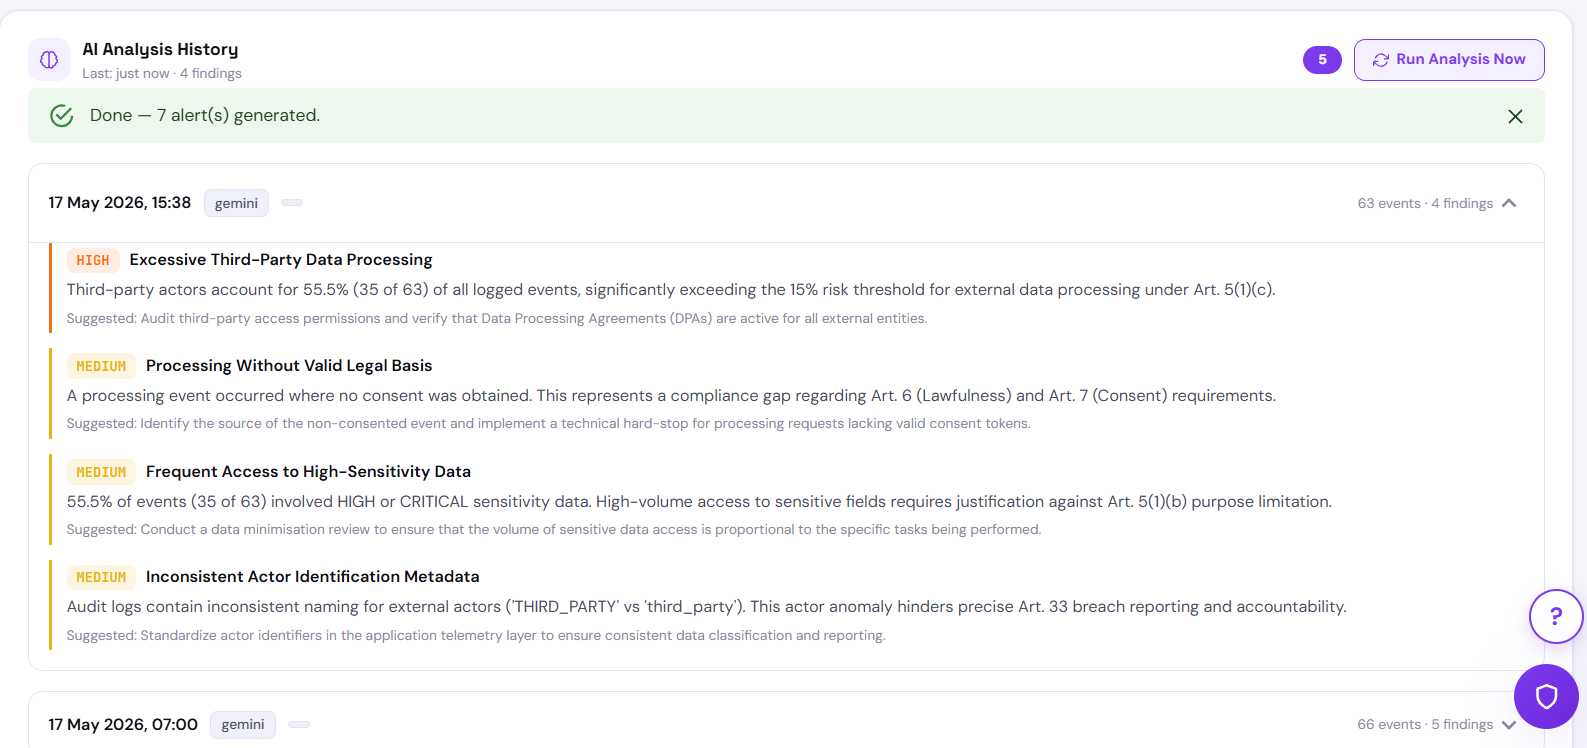
\includegraphics[width=0.95\textwidth]{images/risk-alerts.png}
    \caption{AI-generated risk alerts page showing severity-coded findings with GDPR article citations}
    \label{fig:risk-alerts}
\end{figure}

\subsection{Consent Management}

The \texttt{ConsentsModule} manages GDPR Article 7 consent at the level of individual data processing categories.
Seven categories are defined: \texttt{AD\_TARGETING}, \texttt{DATA\_BROKERING}, \texttt{ANALYTICS}, \texttt{PERSONALISATION}, \texttt{RESEARCH}, \texttt{MARKETING}, and \texttt{THIRD\_PARTY\_SHARING}.

A user can retrieve their current consent settings via \texttt{GET /api/consents/:userId} and update them via \texttt{POST /api/consents}.
Consent records are upserted: a new record is created if none exists, or the existing record is updated.
Events in the audit feed for which the user has withdrawn consent (i.e.\ \texttt{user\_opted\_out} = true) are visually highlighted in the DataGuard dashboard.

Each consent change is recorded with a timestamp, creating a consent history that can be used to verify the state of a user's consent at any point in the past.
This is relevant to GDPR Article 7(1), which requires that the controller be able to demonstrate that the data subject has given consent.
A downloadable consent receipt is generated for each change, providing a portable record that the user can retain as evidence of what they consented to and when.
The combination of the consent history and the consent receipt addresses the accountability requirement of GDPR Article 5(2), which places the burden of proof for compliance on the data controller.

\subsection{Privacy Health Score}

The \texttt{GET /api/dashboard/privacy-score} endpoint returns a 0--100 score that quantifies the privacy posture of a tenant's data access activities.
The score is computed from five weighted factors: the proportion of events with consent obtained, the proportion of events without third-party involvement, the proportion of events at LOW or MEDIUM sensitivity, the absence of active breach reports, and the chain verification status.
The score is displayed on the DataGuard dashboard as an SVG gauge widget.

\subsection{Breach Notification Simulation}

The \texttt{BreachModule} implements a simulation of the GDPR Article 33 breach notification process.
When a breach report is created via \texttt{POST /api/dashboard/breach-report}, the system records the breach timestamp and computes a 72-hour regulatory notification deadline.
The DataGuard dashboard displays a prominent banner showing the elapsed time, the remaining time, and a ``Notify Regulator'' button.
If the deadline is exceeded without action, the banner changes to indicate that the regulatory window has been missed.

\subsection{Webhook System}

The \texttt{WebhooksModule} allows tenant administrators to register endpoint URLs that receive POST notifications when a HIGH or CRITICAL risk alert is generated.
Each webhook delivery includes an \texttt{X-Signature-256} HMAC-SHA256 header, computed from the webhook payload and a shared secret.
The recipient can verify this signature to confirm that the notification came from the audit service.
Delivery uses \texttt{AbortSignal.timeout(8000)} to ensure that slow or unreachable webhook endpoints do not block the risk alert processing pipeline.

\subsection{PDF Compliance Report}

The \texttt{GET /api/dashboard/compliance-report/download} endpoint generates an A4 PDF document using the pdfkit library.
The report includes a summary of the user's audit events, the current retention policy, the hash chain verification status, and a list of the GDPR rights available to the user (access, erasure, portability).
This document is suitable for use as evidence of compliance.

\section{Frontend: DataGuard Privacy Dashboard (React)}

The DataGuard dashboard is a single-page application built with React 18 and TypeScript.
React Router v6 handles client-side routing.
An Axios instance in \texttt{src/api/client.ts} attaches the Bearer token to all API requests via a request interceptor.
All dashboard routes are protected by a \texttt{PrivateRoute} component that redirects unauthenticated users to the login page.

\subsection{Key Components}

The dashboard is composed of the components listed in Table~\ref{tab:components}.

\begin{table}[h]
    \begin{center}
        \begin{tabularx}{\textwidth}{|l|X|}
            \hline
            \textbf{Component} & \textbf{Responsibility} \\
            \hline
            \texttt{Header} & Application title, live status indicator, logout button \\
            \hline
            \texttt{StatsBar} & Four summary statistics cards: total events, high-risk events, third-party events, opted-out events \\
            \hline
            \texttt{SensitivityChart} & Donut chart of event distribution by sensitivity level (Recharts) \\
            \hline
            \texttt{DataFieldsChart} & Bar chart of the most frequently accessed data field categories (Recharts) \\
            \hline
            \texttt{EventFeed} & Chronological timeline of audit events with expand/collapse per event \\
            \hline
            \texttt{EventCard} & Single event card showing action, actor, data fields, reason, and sensitivity badge \\
            \hline
            \texttt{AIChatPanel} & Real-time chat with AI; the user's last 20 events are prepended as context \\
            \hline
            \texttt{RiskAlerts} & AI-generated risk alert cards with severity colour coding \\
            \hline
            \texttt{GDPRControls} & Export and deletion request buttons with status tracking and consent toggles \\
            \hline
            \texttt{PrivacyScore} & SVG gauge showing the 0--100 privacy health score with factor breakdown \\
            \hline
            \texttt{BreachBanner} & Prominent banner showing the GDPR Article 33 72-hour countdown if a breach is active \\
            \hline
        \end{tabularx}
    \end{center}
    \caption{Key React components of the DataGuard privacy dashboard}
    \label{tab:components}
\end{table}

Figure~\ref{fig:dataguard-dashboard} shows the DataGuard privacy dashboard as seen by an authenticated end user.
The overview section displays the four statistics cards, the sensitivity donut chart, the data fields bar chart, and the live event feed.
The privacy health score gauge is visible on the right, providing an at-a-glance summary of the tenant's data access posture.

\begin{figure}[H]
    \centering
    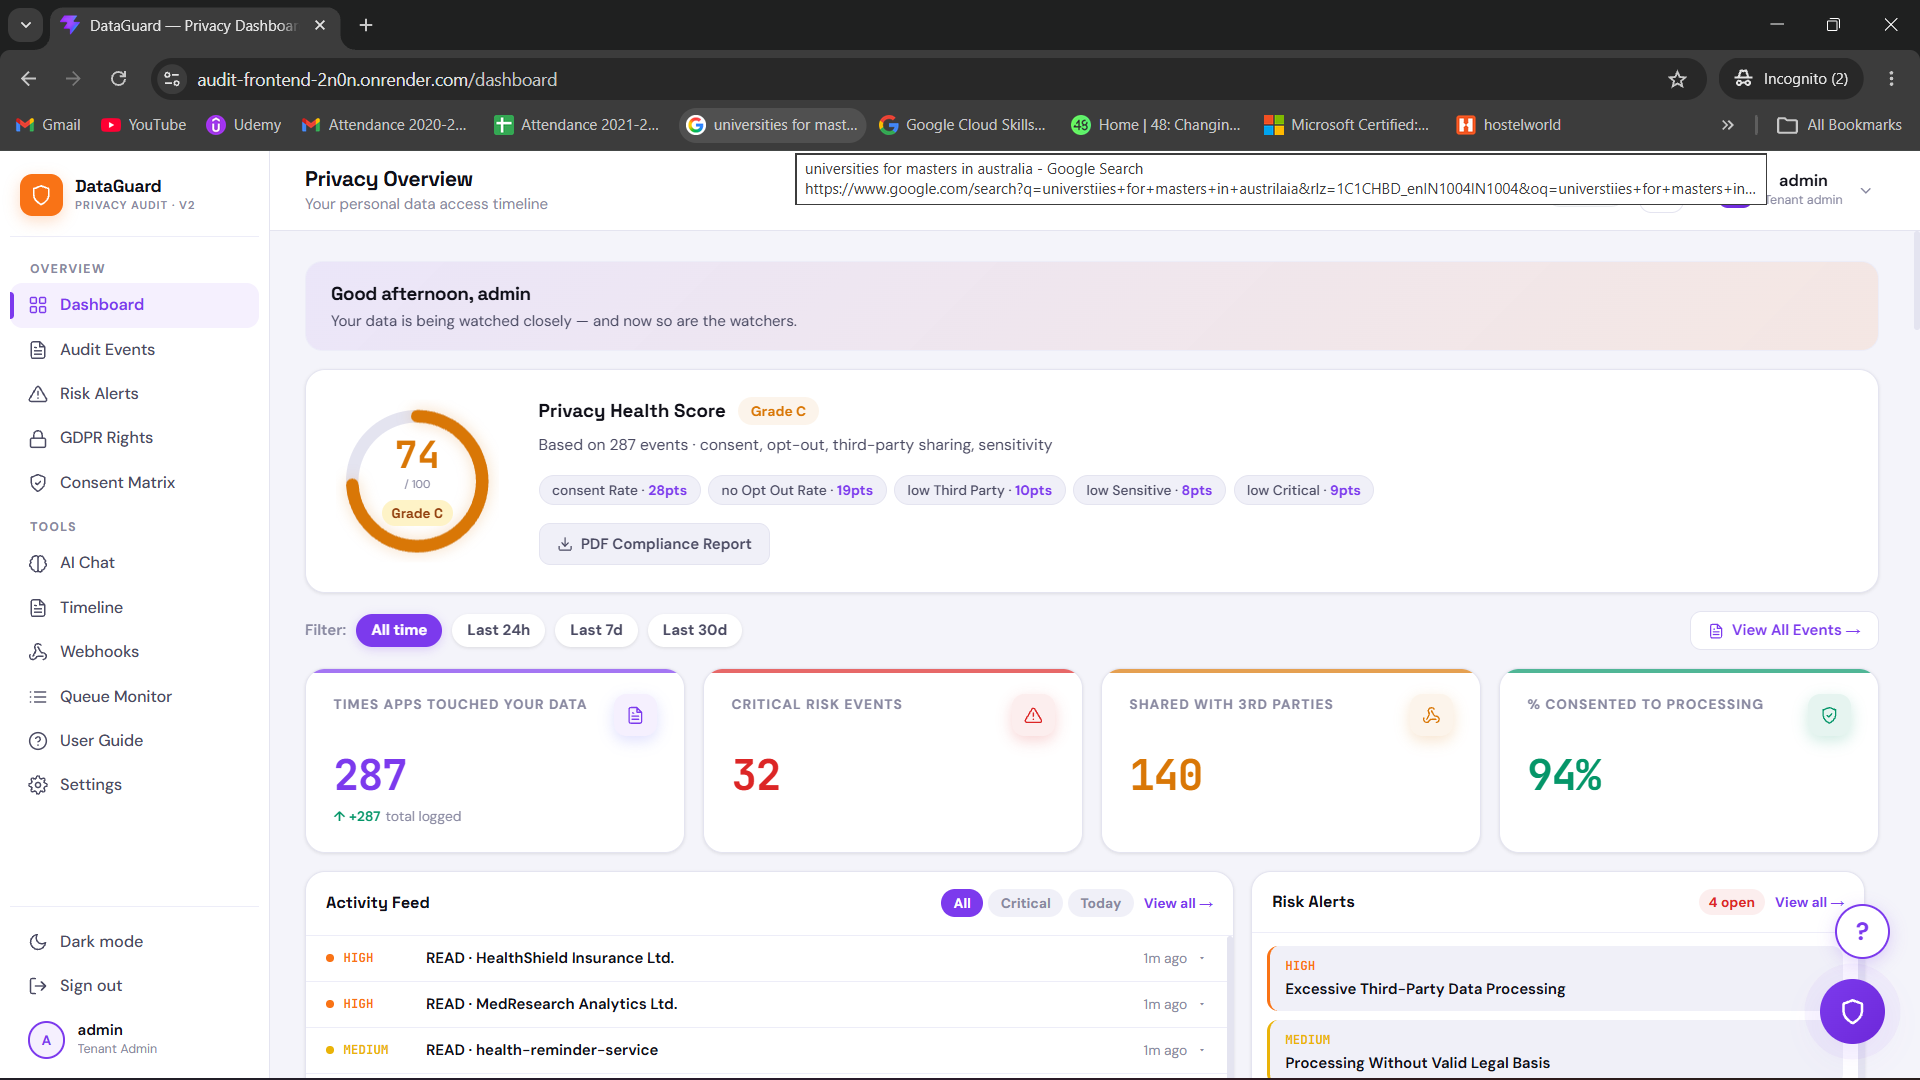
\includegraphics[width=0.95\textwidth]{images/dataguard-dashboard.png}
    \caption{DataGuard privacy dashboard showing the audit event feed, statistics, and privacy health score}
    \label{fig:dataguard-dashboard}
\end{figure}

\subsection{GDPR Controls Interface}

The dashboard exposes two primary GDPR controls to the user.
The ``Request my data export'' button calls \texttt{POST /api/dashboard/exports}.
The frontend then polls \texttt{GET /api/dashboard/exports/:id} every three seconds.
When the status transitions to \texttt{completed}, the browser automatically triggers a file download.
This removes the need for the user to manually check back.

The ``Request account deletion'' button opens a two-step confirmation modal.
The user must confirm their intention twice before the \texttt{POST /api/dashboard/deletions} call is made.
This two-step pattern prevents accidental deletions and is consistent with best practices for destructive actions.

\section{HealthTrack Demo Tenant (Go)}

HealthTrack is a demonstration healthcare portal built with Go 1.21, the Gin web framework, and GORM with a PostgreSQL backend.
It seeds three patient accounts and one doctor account on first boot using an idempotent seeder that checks for existing records before inserting.

The doctor can view patient profiles and medical records.
The patient can view their own data, request a GDPR export, request deletion, and navigate to their DataGuard privacy dashboard via the Privacy Settings page.

Table~\ref{tab:health-events} lists the six audit events emitted during normal operation.

\begin{table}[h]
    \begin{center}
        \begin{tabular}{|p{6cm}|l|l|}
            \hline
            \textbf{Trigger} & \textbf{Action} & \textbf{Actor Type} \\
            \hline
            Doctor views patient profile & READ & EMPLOYEE \\
            \hline
            Doctor views patient medical records & READ & EMPLOYEE \\
            \hline
            System sends appointment reminder & READ & SYSTEM \\
            \hline
            Insurance details accessed & READ & SYSTEM \\
            \hline
            Patient requests data export & EXPORT & SYSTEM \\
            \hline
            Patient requests account deletion & DELETE & SYSTEM \\
            \hline
        \end{tabular}
    \end{center}
    \caption{Audit events emitted by the HealthTrack demo application}
    \label{tab:health-events}
\end{table}

Figure~\ref{fig:healthtrack-dashboard} shows the HealthTrack patient dashboard.
The patient can view their medical records and appointments, and navigate to the DataGuard privacy dashboard via the Privacy Settings link, which initiates the handshake token flow.

\begin{figure}[H]
    \centering
    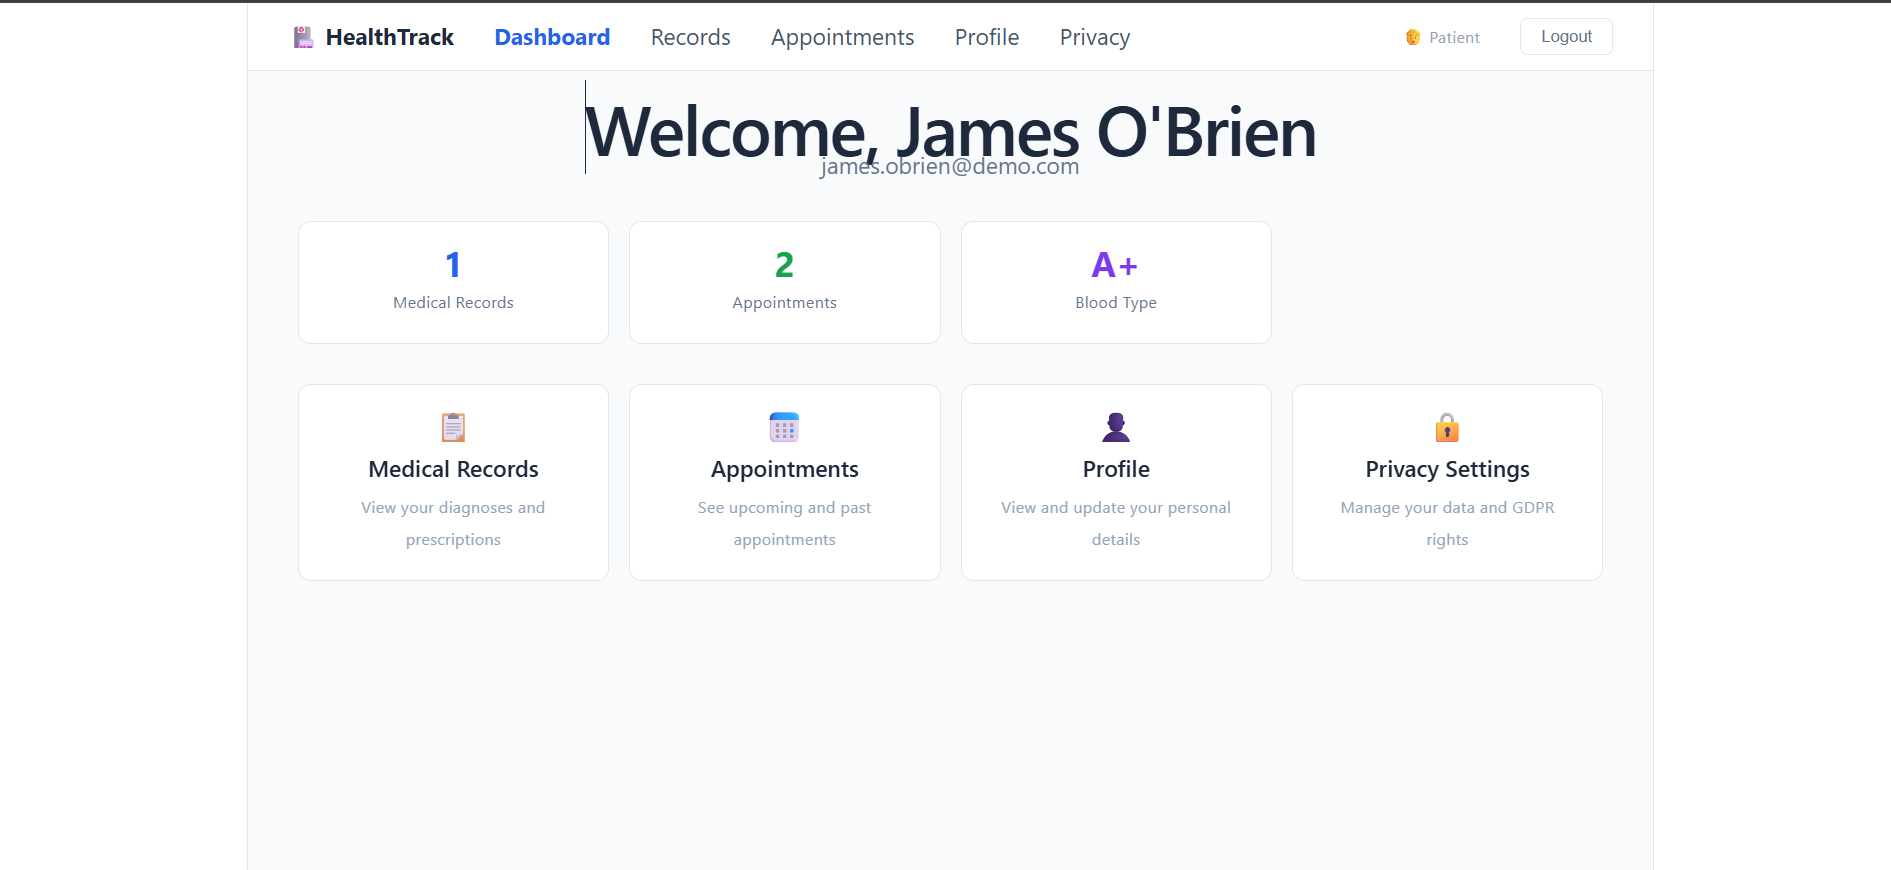
\includegraphics[width=0.95\textwidth]{images/healthtrack-dashboard.png}
    \caption{HealthTrack patient dashboard showing medical records and the privacy settings link}
    \label{fig:healthtrack-dashboard}
\end{figure}

All audit event calls are fire-and-forget.
Each call runs in a goroutine so that a failure or latency in the audit service does not affect the patient's primary healthcare interaction.
Listing~\ref{lst:goaudit} shows the pattern used.

\begin{lstlisting}[language=Go, caption={Fire-and-forget audit event emission in HealthTrack (Go)}, label={lst:goaudit}]
go audit.SendEvent(audit.AuditEvent{
    TenantUserID: patient.UserID.String(),
    Action:       map[string]string{"code": "READ", "label": "Read"},
    DataFields:   []string{"diagnosis", "prescriptions"},
    ActorType:    "EMPLOYEE",
    Sensitivity:  "CRITICAL",
    Reason:       "TREATMENT",
})
\end{lstlisting}

\section{ConnectSocial Demo Tenant (FastAPI)}

ConnectSocial is a demonstration social media platform built with Python 3.11 and FastAPI.
It provides user registration, login, a social feed, post composition, and a privacy settings page.
The application emits seven audit events covering feed algorithm data access, location-based advertising, inter-user data access, third-party analytics, data broker sharing, and GDPR requests.

Table~\ref{tab:social-events} lists the events emitted.

\begin{table}[h]
    \begin{center}
        \begin{tabular}{|p{6cm}|l|l|}
            \hline
            \textbf{Trigger} & \textbf{Action} & \textbf{Actor Type} \\
            \hline
            Feed algorithm reads profile & READ & SYSTEM \\
            \hline
            Ad system reads location data & READ & SYSTEM \\
            \hline
            Another user searches for this user & READ & OTHER\_USER \\
            \hline
            Third-party analytics reads post data & READ & THIRD\_PARTY \\
            \hline
            Check-in data shared with location partner & SHARE & DATA\_BROKER \\
            \hline
            User requests data export & EXPORT & SYSTEM \\
            \hline
            User requests account deletion & DELETE & SYSTEM \\
            \hline
        \end{tabular}
    \end{center}
    \caption{Audit events emitted by the ConnectSocial demo application}
    \label{tab:social-events}
\end{table}

Figure~\ref{fig:connectsocial-dashboard} shows the ConnectSocial user interface.
The social feed, post composition, and privacy settings are visible.
The privacy settings page provides access to the DataGuard dashboard and displays the user's consent preferences.

\begin{figure}[H]
    \centering
    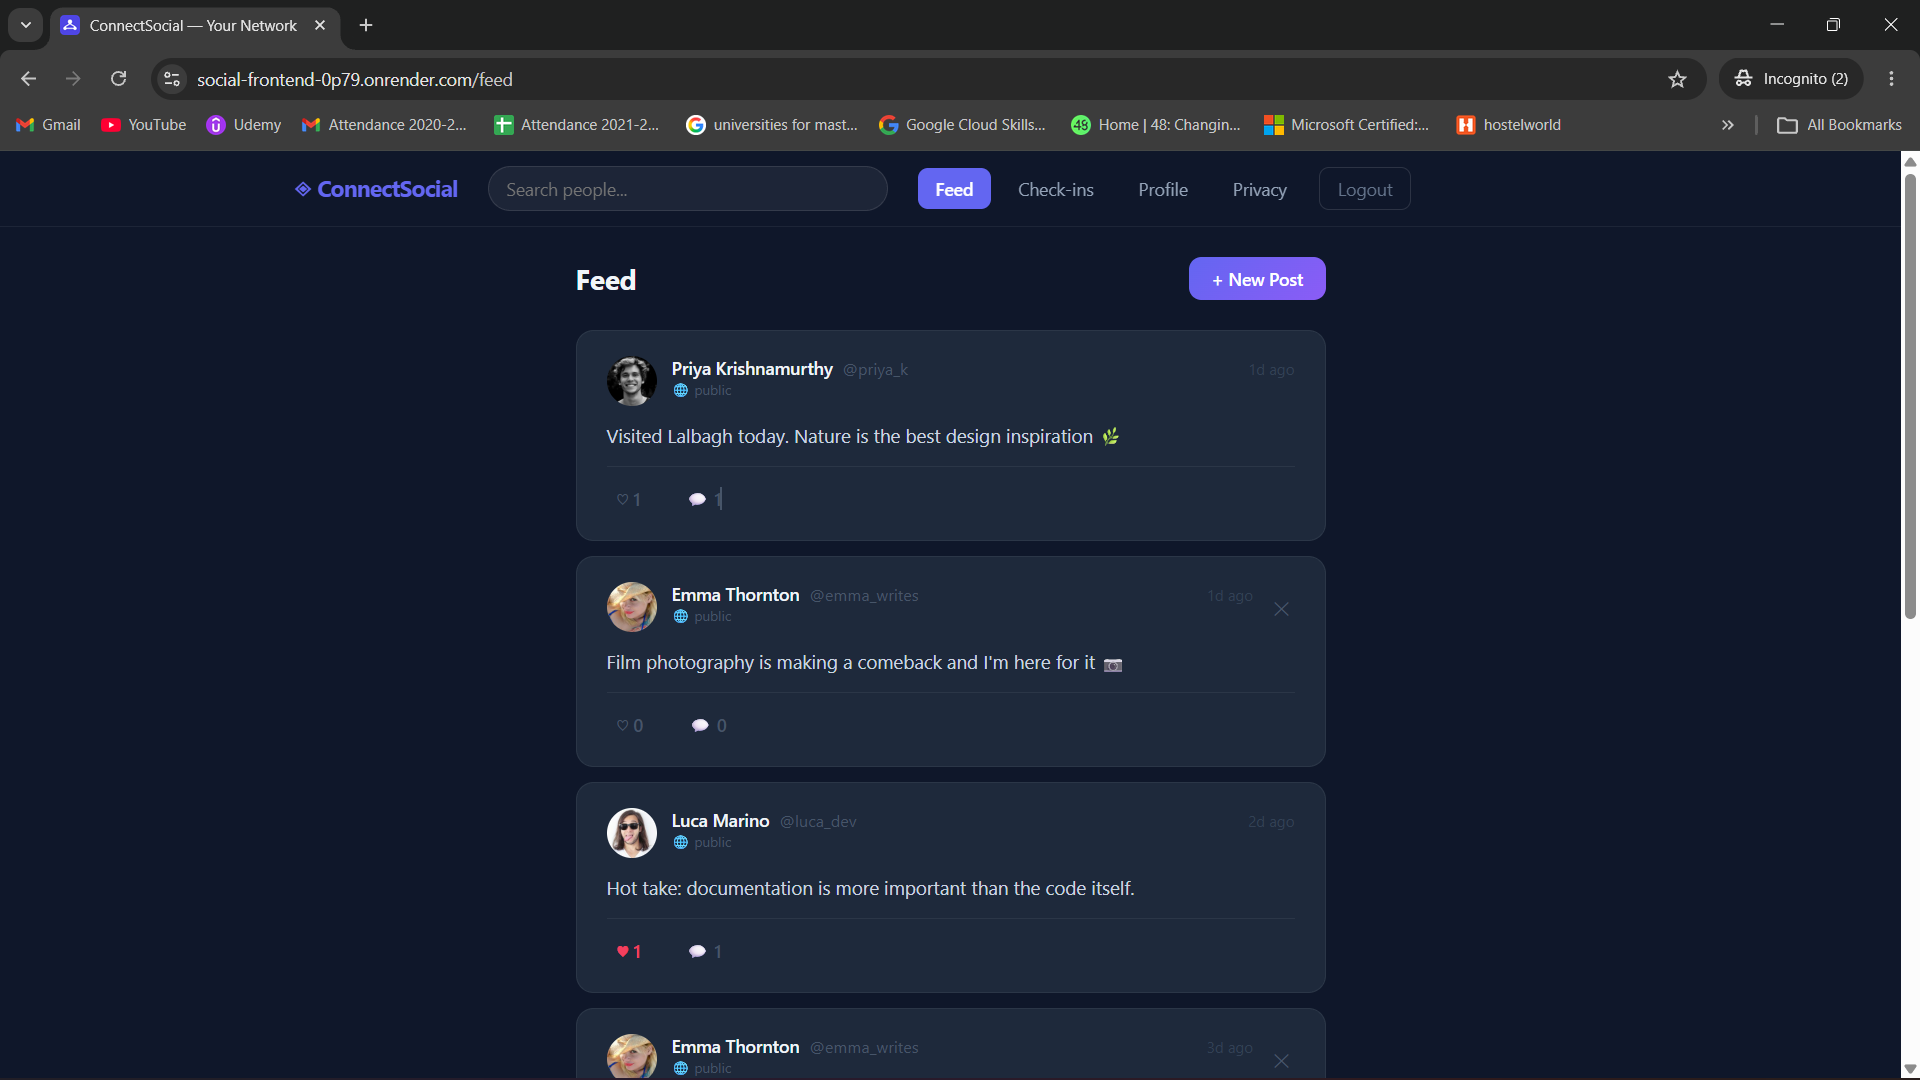
\includegraphics[width=0.95\textwidth]{images/connectsocial-dashboard.png}
    \caption{ConnectSocial social media application showing the user feed and privacy settings page}
    \label{fig:connectsocial-dashboard}
\end{figure}

The Python SDK uses \texttt{httpx} for HTTP communication.
The \texttt{audit.py} module in the ConnectSocial backend wraps each SDK call in a try/except block, logging any exception and continuing, consistent with the fire-and-forget requirement.

\section{SDK Implementation}

\subsection{Go SDK}

The Go SDK provides a \texttt{Client} struct with three methods.
\texttt{Send()} submits an event synchronously and returns any HTTP error.
\texttt{SendAsync()} launches a goroutine and returns immediately.
\texttt{IssueUserToken()} calls the backend's \texttt{POST /api/dashboard/token} endpoint and returns the handshake JWT for a given tenant user ID.
The SDK uses only the Go standard library for HTTP communication and has no external dependencies.

\subsection{Python SDK}

The Python SDK provides an \texttt{AuditClient} class with \texttt{send()} and \texttt{issue\_user\_token()} methods.
All event field types are defined as Python dataclasses, providing type checking at the call site.
The package is distributed as a local Python package using \texttt{setup.py} and is installed with \texttt{pip install -e .}.
Listing~\ref{lst:pysdk} shows a usage example.

\begin{lstlisting}[language=Python, caption={Python SDK usage example in ConnectSocial}, label={lst:pysdk}]
from privacy_audit_sdk import AuditClient, AuditEvent
client = AuditClient(api_key=API_KEY, service_url=SERVICE_URL)
client.send(AuditEvent(
    tenant_user_id=str(user.id),
    action="SHARE",
    data_fields=["location", "checkin_data"],
    actor_type="DATA_BROKER",
    sensitivity="HIGH",
    reason="DATA_BROKERING",
    consent_obtained=False,
))
\end{lstlisting}

\subsection{TypeScript SDK}

The TypeScript SDK provides an \texttt{AuditClient} class using the native \texttt{fetch} API, which requires no runtime dependencies.
Full TypeScript type definitions are exported for all event fields.
The SDK supports both \texttt{send()} for synchronous calls and \texttt{sendAsync()} for non-blocking calls using a \texttt{Promise} without \texttt{await}.

\section{Infrastructure}

The full platform is containerised using Docker Compose.
The configuration defines nine services: \texttt{audit-backend}, \texttt{audit-frontend}, \texttt{health-backend}, \texttt{health-frontend}, \texttt{social-backend}, \texttt{social-frontend}, \texttt{postgres} (for the audit service), \texttt{redis}, and \texttt{mongo}.
Two additional PostgreSQL containers (\texttt{postgres-health}, \texttt{postgres-social}) serve the tenant databases.
All services communicate over a shared Docker network named \texttt{audit-network}.

Health checks are configured on the PostgreSQL and Redis services.
All services that depend on them use \texttt{depends\_on: condition: service\_healthy} so that they wait for the underlying services to be ready before starting.
This prevents connection failures during the multi-container startup sequence.

An nginx reverse proxy routes requests from named local hostnames to the appropriate frontend services.
The \texttt{dataguard.local} hostname routes to the audit frontend.
The \texttt{health.local} hostname routes to the HealthTrack frontend.
The \texttt{social.local} hostname routes to the ConnectSocial frontend.
A one-time \texttt{setup-hosts.sh} script adds these entries to the host machine's \texttt{/etc/hosts} file.

A \texttt{start.sh} script orchestrates the full startup sequence: it checks that Docker is running, copies the environment file if absent, runs Docker Compose, and prints a health status table with all service URLs and port numbers.
A \texttt{Makefile} provides shortcut commands for starting, stopping, resetting, and viewing logs for the platform.

The nginx reverse proxy configuration deserves particular mention as a developer experience decision.
Without named hostnames, developers must remember that the DataGuard dashboard is at \texttt{localhost:3000}, the audit API is at \texttt{localhost:8080}, and the tenant applications are at ports 3001 and 3002.
The nginx proxy, combined with a one-time \texttt{setup-hosts.sh} script that adds entries to the host machine's \texttt{/etc/hosts} file, replaces these numeric ports with memorable hostnames: \texttt{dataguard.local}, \texttt{health.local}, and \texttt{social.local}.
This configuration also mirrors a realistic production deployment, where each service is addressed by a subdomain rather than a port number.
The nginx configuration for each frontend service uses \texttt{try\_files \$uri /index.html} to support client-side routing, which is required for React Router to handle direct URL navigation correctly within each single-page application.

\section{Implementation Challenges}

\subsection{Hash Chain Concurrency Under Concurrent Submissions}

The hash chain computation requires fetching the most recent event before saving the new one.
Under concurrent event submissions from the same tenant and user, two processors could read the same most-recent event and produce two events with the same \texttt{prev\_hash}.
This would break the chain integrity.

The solution was to use BullMQ's job grouping feature to serialise processing per \texttt{(tenantId, tenantUserId)} pair.
Events for the same user are placed in a named queue group and processed strictly in FIFO order.
This serialisation is transparent to the SDK caller and does not affect throughput at the tenant level.

\subsection{Docker Service Startup Order}

The PostgreSQL and Redis services require several seconds to become ready after their containers start.
Without health checks, NestJS and other backend services attempted to connect before the databases were accepting connections, resulting in startup crashes.
Health check commands were added to the PostgreSQL services (\texttt{pg\_isready}) and the Redis service (\texttt{redis-cli ping}).
All dependent services were updated with \texttt{depends\_on: condition: service\_healthy}.

\subsection{Cross-Origin Resource Sharing (CORS)}

The system involves multiple cross-origin request combinations.
The DataGuard frontend at \texttt{dataguard.local} calls the audit backend at \texttt{api.dataguard.local}.
The HealthTrack frontend at \texttt{health.local} calls the HealthTrack backend.
CORS configuration required explicit origin whitelisting in each backend service.
In the NestJS backend, the allowed origins are read from environment variables, enabling the same Docker Compose file to work in both local development (using \texttt{.local} hostnames) and cloud deployment (using Render URLs).

\subsection{Vite Environment Variable Injection}

React applications built with Vite embed environment variables at build time, not at runtime.
During early development, \texttt{VITE\_API\_URL} was placed in the Docker Compose \texttt{environment:} section, which sets runtime environment variables.
These runtime variables are not available to the Vite build process.

The fix was to move \texttt{VITE\_API\_URL} to the Docker Compose \texttt{build: args:} section and to read it in the \texttt{Dockerfile} as a build argument passed to the Vite build command.
This ensured that the correct API URL was embedded in the compiled JavaScript bundle.

\subsection{TypeORM Schema Evolution Across Development Phases}

The project used TypeORM's \texttt{synchronize: true} option during development to apply schema changes automatically on startup.
Several significant schema additions were made across phases: the \texttt{prev\_hash} and \texttt{hash} columns added in Phase 2, the \texttt{dashboard\_users} and \texttt{linked\_accounts} tables added in Phase 5, and the \texttt{consents}, \texttt{breach\_reports}, and \texttt{webhooks} tables added in Phase 14.
Careful management of Docker volumes was required to ensure that existing development data was not lost during each phase transition.


% ============================================================
% CHAPTER 6: TESTING AND EVALUATION
% ============================================================
\chapter{Testing and Evaluation}

\section{Testing Strategy}

The testing approach combined end-to-end functional testing across the full platform stack, API-level testing through the Swagger UI, and informal user evaluation with peers acting in specific user roles.
Automated unit tests were written for selected utility functions (including the hash computation and the privacy score calculation), but the primary validation method was manual end-to-end scenario testing in the running Docker Compose environment.

The decision to prioritise end-to-end testing over unit testing reflects the nature of the system.
The most significant risks in the system are integration risks: whether the queue processor correctly computes the hash chain, whether the export workflow correctly transitions through states, and whether the handshake token flow correctly pre-authenticates the user in DataGuard.
These risks are best tested at the integration level.

\section{Functional Testing}

Functional testing verified that each system feature behaved according to its specification.
Test scenarios were drawn from the progress tracker task list, which tracked 174 individual tasks across 14 phases.
No task was marked complete until the corresponding feature was verified to work correctly in the running environment.

Table~\ref{tab:test-scenarios} lists the key test scenarios and their outcomes.

\begin{longtable}{|p{4cm}|p{6.5cm}|c|}
    \caption{Key functional test scenarios and results}
    \label{tab:test-scenarios} \\
    \hline
    \textbf{Scenario} & \textbf{Description} & \textbf{Result} \\
    \hline
    \endfirsthead
    \hline
    \textbf{Scenario} & \textbf{Description} & \textbf{Result} \\
    \hline
    \endhead
    \hline
    \multicolumn{3}{r}{\small\textit{Continued on next page}} \\
    \endfoot
    \hline
    \endlastfoot
    Tenant registration & Tenant registers via API, receives API key, sends test event & Pass \\
    \hline
    Event ingestion & SDK sends event, queue processes it, event visible in dashboard & Pass \\
    \hline
    Idempotency & Same event\_id submitted twice, second submission rejected & Pass \\
    \hline
    Hash chain verification & Chain verify endpoint returns clean after 20 events seeded & Pass \\
    \hline
    Chain tamper detection & Event hash manually altered, verify-chain returns 400 & Pass \\
    \hline
    Data export & User requests export, polls status, downloads JSON file & Pass \\
    \hline
    Export expiry & Export link accessed after 24-hour expiry returns 410 & Pass \\
    \hline
    Data deletion & User requests deletion, events removed, evidence hash stored & Pass \\
    \hline
    Retention cron & Cron triggered manually, events older than retention window deleted & Pass \\
    \hline
    AI risk analysis & Cron triggered manually, Claude API returns findings, alerts visible & Pass \\
    \hline
    Google OAuth & User signs in with Google, arrives at DataGuard dashboard authenticated & Pass \\
    \hline
    Handshake token flow & HealthTrack ``View my privacy'' button opens DataGuard pre-authenticated & Pass \\
    \hline
    Consent management & User toggles consent off, opted-out events highlighted in feed & Pass \\
    \hline
    Webhook delivery & Risk alert triggers HMAC-signed delivery to registered endpoint & Pass \\
    \hline
    PDF compliance report & User downloads A4 PDF report containing event summary & Pass \\
    \hline
    Breach notification & Breach report created, 72-hour countdown visible on dashboard & Pass \\
    \hline
    Privacy health score & Score computed and displayed as gauge on dashboard & Pass \\
    \hline
    Rate limiting & 11 rapid requests to /events from same IP returns 429 & Pass \\
    \hline
\end{longtable}

All 18 key scenarios passed.
The tamper detection test, where a hash was manually altered in the database and the verify-chain endpoint was called, confirmed that the cryptographic integrity mechanism works as intended.

\section{API Testing}

The Swagger UI at \texttt{http://api.dataguard.local/api/docs} was used to test individual API endpoints.
It was generated automatically by the \texttt{@nestjs/swagger} module and includes all request schemas, response schemas, and authentication requirements.
The Swagger UI was particularly useful for testing the export and deletion workflow endpoints, which involve state transitions that are difficult to trigger by other means.

A \texttt{demo-onboard.sh} script was written to exercise the full tenant onboarding flow programmatically using curl commands.
The script registers a tenant, sends five events, and prints the dashboard URL.
This script was used for smoke testing the system after each significant change and confirmed that the end-to-end event pipeline was working correctly.

The developer tools module (\texttt{DevModule}) provided manual trigger endpoints for the risk analysis cron, retention cron, weekly email digest, and event seeding.
These were used extensively during testing to exercise the asynchronous workflows without waiting for the scheduled cron intervals.

\section{User Evaluation}

An informal user evaluation was conducted with a group of peers.
The purpose of the evaluation was to assess the usability of the system from the perspective of each user role: a patient in a healthcare application, a user of a social media application, and a developer integrating the service into a new application.

\subsection{Participant Roles and Tasks}

Three participant roles were used, each with a defined set of tasks.

The first role was a patient user.
The participant logged into HealthTrack as James O'Brien, navigated to their patient dashboard, reviewed their medical records, clicked ``View my privacy'', arrived at the DataGuard dashboard without a second login, reviewed the audit trail of data accesses, and requested a GDPR data export.

The second role was a social media user.
The participant logged into ConnectSocial as Emma Thornton, browsed the social feed, and navigated to the privacy settings page.
They were asked to find out whether their location data had been shared with any third parties, and to opt out of ad targeting.

The third role was a tenant developer.
The participant followed the tenant onboarding wizard: they registered a new tenant account, copied the generated API key, and used the provided curl command in the wizard to send a test event.
They then opened the DataGuard dashboard to verify that the event appeared.

\subsection{Findings}

The evaluation produced the following observations.

The patient user found the audit event timeline intuitive.
The sensitivity colour-coding --- Critical in red, High in orange, Medium in yellow, Low in green --- was the feature most consistently identified as useful.
The participant noted that they had not previously been aware that a healthcare application could share insurance data with a separate billing system, and that seeing this in the audit trail was informative.
The handshake token flow, where clicking ``View my privacy'' opened DataGuard without a second login, was completed without any issues.

The social media user successfully located the events showing location data access.
The ad targeting opt-out toggle on the consent management section was found and used without guidance.
The user noted that the consent category label ``AD\_TARGETING'' was slightly technical and would benefit from a plain-language description such as ``Used for showing you targeted advertisements''.

The tenant developer role was completed in under five minutes.
The auto-generated curl command in the onboarding wizard was the feature identified as most valuable.
The participant noted that without the sample curl command, knowing the exact JSON structure required by the API would have taken considerably longer to determine.

\subsection{Areas for Improvement}

The evaluation identified three areas for future improvement.
The AI chat interface experienced response latency of two to five seconds due to the Claude API round-trip time.
A typing indicator while the model is processing would improve the perceived responsiveness.
The consent category labels, as noted above, would benefit from plain-language descriptions.
The ``View my privacy'' link in HealthTrack currently opens the DataGuard dashboard in a new browser tab, which requires the user to context-switch between the healthcare application and the privacy dashboard.
An embedded iframe approach would provide a more integrated experience.

Despite these areas for improvement, the overall reception of the system during evaluation was positive.
All three participant roles completed their assigned tasks without external assistance.
The patient role participant expressed that the audit trail provided a level of transparency they had not previously experienced from a healthcare application, and that the ability to request a data export in a single click was more straightforward than expected.
The developer role participant noted that the onboarding wizard's auto-generated curl command removed what they described as the most common friction point in API integration: knowing the exact request format without reading the full documentation.
These observations, while informal, suggest that the system's core design decisions --- the seamless handshake token flow, the structured event format, and the developer-facing onboarding tooling --- are well-aligned with the needs of their respective user groups.

\section{Evaluation Against Requirements}

Table~\ref{tab:requirements-eval} evaluates the implemented system against the eleven functional requirements defined in Chapter~Four.

\begin{table}[h]
    \begin{center}
        \begin{tabular}{|c|p{9cm}|c|}
            \hline
            \textbf{Req.} & \textbf{Requirement} & \textbf{Status} \\
            \hline
            FR-1 & Multi-tenant support with data isolation & Met \\
            \hline
            FR-2 & REST API for event submission with API key authentication & Met \\
            \hline
            FR-3 & Tamper-evident SHA-256 hash-chained audit log & Met \\
            \hline
            FR-4 & Chain integrity verification endpoint & Met \\
            \hline
            FR-5 & User privacy dashboard & Met \\
            \hline
            FR-6 & GDPR Article 20 export workflow with expiring links & Met \\
            \hline
            FR-7 & GDPR Article 17 deletion workflow with evidence storage & Met \\
            \hline
            FR-8 & Per-tenant retention policy with automated cron cleanup & Met \\
            \hline
            FR-9 & AI risk agent with anomaly detection and alert storage & Met \\
            \hline
            FR-10 & SDKs in Go, Python, and TypeScript & Met \\
            \hline
            FR-11 & Two integrated demo tenant applications & Met \\
            \hline
        \end{tabular}
    \end{center}
    \caption{Evaluation of the implemented system against all functional requirements}
    \label{tab:requirements-eval}
\end{table}

As shown in Table~\ref{tab:requirements-eval}, all eleven functional requirements were met.
The system also delivered seven features beyond the original requirements: consent management (GDPR Article 7), breach notification simulation (GDPR Article 33), a webhook system with HMAC-signed delivery, a PDF compliance report generator, a privacy health score, a multi-provider AI orchestration layer, and an interactive tenant onboarding wizard.
These additional features were implemented in Phases 13 and 14 and increase the demonstration value and academic complexity of the project.

The non-functional requirements were also evaluated during testing.
The 202 Accepted response time requirement (NFR-1) was consistently met: because the event is placed on the BullMQ queue rather than written directly to the database, the HTTP response is returned before the hash chain computation occurs, keeping the response time well within 100 milliseconds under the tested load.
The multi-level tenancy isolation (NFR-2) was verified by attempting to access one tenant's events using a second tenant's API key --- the request was correctly rejected with a 403 response at the middleware layer.
The single-command deployment requirement (NFR-3) was satisfied by the \texttt{docker compose up --build} command, which successfully brought all nine services to a healthy state in under five minutes on a standard development machine.


% ============================================================
% CHAPTER 7: CONCLUSIONS AND FUTURE WORK
% ============================================================
\chapter{Conclusions and Future Work}

\section{Conclusions}

This project set out to build a reusable, multi-tenant Privacy Audit and Data Transparency Service that bridges the gap between regulatory intent and practical user-facing privacy transparency.
The system was fully implemented, completing 174 planned tasks across 14 development phases.
All eleven functional requirements were met, and the system passed all 18 key functional test scenarios.

The central contribution of the project is the combination of a developer-facing audit SDK and a user-facing privacy dashboard, connected through a secure, tamper-evident event store.
The hash chain implementation, based on the technique introduced by Haber and Stornetta \cite{hashchain}, ensures that the audit log cannot be retroactively modified without detection.
The three-tier authentication architecture cleanly separates the security requirements of machine clients, admin users, and end users.

The GDPR compliance features --- export, deletion, consent management, retention enforcement, and breach notification --- demonstrate the application of the regulation across multiple articles in a single integrated platform.
The AI risk agent, powered by the Claude API, provides automated compliance monitoring without requiring manual review of every event.

The multi-tenant architecture was validated through two distinct demo applications built with different technology stacks (Go and Python), demonstrating that the platform integrates with heterogeneous environments.
The five-layer architecture, the shared-database multi-tenancy model described by Walraven et al.\ \cite{walraven2011}, and the three-level isolation enforcement provide a template for how privacy-by-design \cite{cavoukian2009} can be operationalised in a production-grade SaaS system.

The choice to build two demo applications in deliberately different languages --- Go for HealthTrack and Python for ConnectSocial --- was made to demonstrate that the SDK abstraction is genuinely language-agnostic.
A healthcare operator and a social media operator represent different sectors, different data sensitivity profiles, and different technology ecosystems.
The fact that both integrate with DataGuard through the same canonical event format, and that users from both applications can access a unified privacy dashboard, validates the reusability claim in the dissertation title.
The SDKs reduce the integration to a consistent two-step process regardless of the tenant's technology stack: initialise a client with the API key and service URL, then call \texttt{send()} or \texttt{sendAsync()} with the event fields.
This simplicity was a deliberate design goal and was confirmed by the developer evaluation participant, who completed the full onboarding flow in under five minutes.

The informal user evaluation confirmed that the core user flows --- viewing the audit trail, requesting a data export, and opting out of data categories --- were understandable and usable without prior training.
The seamless handshake token flow, which removes the need for a second login when navigating from a tenant application to DataGuard, was particularly well-received.

\section{Limitations}

Several limitations of the current implementation are acknowledged.

The system was tested with seed data and manually triggered events.
Performance under high-throughput production load was not formally benchmarked.
The hash chain serialisation per tenant user, while correct, introduces a sequential bottleneck for very high-frequency event submissions from the same user.

The informal user evaluation used a small group of peers rather than a formal user study with a diverse, representative sample.
The findings are indicative but not statistically significant.

The AI risk agent's analysis quality depends on the system prompt engineering and the behaviour of the underlying language model.
The agent's findings should be reviewed by a qualified privacy professional before being acted upon in a production environment.

The system has not been subjected to a formal security audit.
The API key authentication, JWT signing configuration, CORS policy, and HMAC webhook verification should all be reviewed by a security specialist before the system is deployed with real personal data.

The consent management implementation operates at the data category level, which is a simplification relative to the full requirements of GDPR Article 7.
A production-grade implementation would require consent to be recorded at the level of individual processing purposes, with explicit timestamps, version identifiers for the consent notice shown to the user, and a mechanism for re-obtaining consent when the processing purpose changes.
The current implementation demonstrates the architectural pattern but does not yet meet the evidentiary standard that a data protection authority would expect in a formal compliance audit.

\section{Future Work}

Several directions for future development are identified.

A formal performance benchmarking study would quantify the throughput and latency of the event ingestion pipeline under realistic concurrent load.
This would enable an evidence-based decision about whether additional optimisation, such as database connection pooling tuning or horizontal scaling of the queue processors, is required.

SDK Mode 3 (direct queue publish via Kafka or RabbitMQ) was deferred from the original design.
Implementing this mode would complete the SDK feature set and make the platform suitable for high-throughput tenants who require the most resilient integration pattern.

The consent management module currently operates at the data category level.
A more granular implementation could manage consent at the level of individual data fields and specific processing purposes, providing users with finer-grained control.

The AI risk agent uses a single-turn prompt approach.
A multi-turn analysis conversation, where the model can request additional event details and access historical analysis context, would improve the quality of risk findings.
A formal evaluation of the agent's precision and recall against a labelled dataset of known GDPR violations would provide a quantitative measure of its effectiveness.

A formal security audit, including penetration testing of the API authentication endpoints, JWT configuration, and webhook HMAC verification, would be required before deploying the system with real personal data.
Additionally, cloud deployment to a managed platform such as Render or AWS, with proper secret management, would demonstrate the system's production readiness.

Finally, the multi-tenant account linking feature --- where a user who has accounts in both HealthTrack and ConnectSocial can view a unified privacy dashboard across both tenants --- is partially implemented in the backend but not yet wired to the frontend.
Completing this feature would demonstrate cross-tenant identity aggregation, which is a compelling use case for users of multiple connected applications.


% ============================================================
% BIBLIOGRAPHY
% ============================================================
\bibliographystyle{plain}
\bibliography{references}


% ============================================================
% APPENDICES
% ============================================================
\appendix

\chapter{Database Schema Reference}

This appendix provides the full PostgreSQL schema for the core tables of the Privacy Audit Service.

\section{\texttt{tenants} Table}

\begin{longtable}{|l|l|p{6cm}|}
    \caption{Full schema for the \texttt{tenants} table} \label{tab:tenants-schema} \\
    \hline
    \textbf{Column} & \textbf{Type} & \textbf{Notes} \\
    \hline
    \endfirsthead
    \hline
    \textbf{Column} & \textbf{Type} & \textbf{Notes} \\
    \hline
    \endhead
    id & UUID PK & Auto-generated (\texttt{gen\_random\_uuid()}) \\
    \hline
    name & VARCHAR(255) & Tenant display name \\
    \hline
    email & VARCHAR UNIQUE & Primary contact email \\
    \hline
    api\_key\_hash & VARCHAR(64) & SHA-256 hash of the API key \\
    \hline
    retention\_days & INT & Default 90 days \\
    \hline
    is\_active & BOOLEAN & Default true; set false to disable tenant \\
    \hline
    created\_at & TIMESTAMP & Auto-set on insert \\
    \hline
\end{longtable}

\section{\texttt{audit\_events} Table}

\begin{longtable}{|l|l|p{6cm}|}
    \caption{Full schema for the \texttt{audit\_events} table} \label{tab:events-schema} \\
    \hline
    \textbf{Column} & \textbf{Type} & \textbf{Notes} \\
    \hline
    \endfirsthead
    \hline
    \textbf{Column} & \textbf{Type} & \textbf{Notes} \\
    \hline
    \endhead
    id & UUID PK & \\
    \hline
    tenant\_id & UUID FK & References \texttt{tenants.id}, NOT NULL \\
    \hline
    tenant\_user\_id & VARCHAR & User's identifier in the tenant application \\
    \hline
    event\_id & UUID UNIQUE & SDK-generated idempotency key \\
    \hline
    action\_code & VARCHAR(20) & READ, WRITE, SHARE, DELETE, EXPORT, ANALYSE \\
    \hline
    action\_label & VARCHAR(100) & Human-readable label \\
    \hline
    data\_fields & JSONB & Array of field name strings \\
    \hline
    reason\_code & VARCHAR(50) & Data access purpose code \\
    \hline
    reason\_label & VARCHAR(200) & Human-readable reason \\
    \hline
    actor\_type & VARCHAR(20) & SYSTEM, EMPLOYEE, THIRD\_PARTY, DATA\_BROKER \\
    \hline
    actor\_label & VARCHAR(100) & Human-readable actor description \\
    \hline
    actor\_identifier & VARCHAR nullable & Specific actor identifier (e.g., doctor name) \\
    \hline
    sensitivity\_code & VARCHAR(10) & LOW, MEDIUM, HIGH, CRITICAL \\
    \hline
    third\_party\_involved & BOOLEAN & \\
    \hline
    third\_party\_name & VARCHAR nullable & \\
    \hline
    retention\_days & INT & Per-tenant retention window \\
    \hline
    region & VARCHAR(10) nullable & ISO region code (e.g., IE) \\
    \hline
    consent\_obtained & BOOLEAN & \\
    \hline
    user\_opted\_out & BOOLEAN & \\
    \hline
    meta & JSONB nullable & Extensible metadata from tenant \\
    \hline
    prev\_hash & VARCHAR(64) nullable & SHA-256 hash of previous event in chain \\
    \hline
    hash & VARCHAR(64) & SHA-256 hash of this event plus prev\_hash \\
    \hline
    occurred\_at & TIMESTAMP & Event time as reported by the tenant \\
    \hline
    created\_at & TIMESTAMP & Ingestion time (set by backend) \\
    \hline
\end{longtable}

\chapter{SDK Quick-Start Reference}

This appendix provides quick-start code examples for all three SDKs.

\section{Go SDK Usage}

The Go SDK is located at \texttt{privacy-audit-sdk/go/}.
Listing~\ref{lst:gosdk} shows a complete usage example.

\begin{lstlisting}[language=Go, caption={Go SDK initialisation and event submission}, label={lst:gosdk}]
import "github.com/VirtualBeetle/privacy-audit-sdk/go/audit"

client := audit.NewClient(
    os.Getenv("AUDIT_SERVICE_URL"),
    os.Getenv("AUDIT_API_KEY"),
)
err := client.Send(audit.AuditEvent{
    TenantUserId:    userID,
    Action:          "READ",
    DataFields:      []string{"email", "full_name"},
    ActorType:       "EMPLOYEE",
    Sensitivity:     "HIGH",
    Reason:          "TREATMENT",
    ConsentObtained: true,
})
\end{lstlisting}

\section{Python SDK Usage}

The Python SDK is located at \texttt{privacy-audit-sdk/python/}.
Install it with \texttt{pip install -e .} and use it as shown in Listing~\ref{lst:pysdk2}.

\begin{lstlisting}[language=Python, caption={Python SDK event submission}, label={lst:pysdk2}]
from privacy_audit_sdk import AuditClient, AuditEvent
client = AuditClient(api_key=API_KEY, service_url=SERVICE_URL)
client.send(AuditEvent(
    tenant_user_id=str(user.id),
    action="READ",
    data_fields=["location"],
    actor_type="SYSTEM",
    sensitivity="MEDIUM",
    reason="AD_TARGETING",
    consent_obtained=True,
))
\end{lstlisting}

\section{TypeScript SDK Usage}

The TypeScript SDK is located at \texttt{privacy-audit-sdk/js/}.
Listing~\ref{lst:tssdk} shows asynchronous (non-blocking) event submission.

\begin{lstlisting}[language=JavaScript, caption={TypeScript SDK non-blocking event submission}, label={lst:tssdk}]
import { AuditClient } from '@virtualbeetle/privacy-audit-sdk';
const client = new AuditClient({
  apiKey: process.env.AUDIT_API_KEY,
  serviceUrl: process.env.AUDIT_SERVICE_URL,
});
client.sendAsync({
  tenantUserId: userId,
  action: 'SHARE',
  dataFields: ['email', 'purchase_history'],
  actorType: 'DATA_BROKER',
  sensitivity: 'HIGH',
  reason: 'DATA_BROKERING',
  consentObtained: false,
});
\end{lstlisting}

\end{document}
